\documentclass[aps,prb,reprint,amsmath,amssymb,floatfix]{revtex4-2}
\usepackage{graphicx}
\usepackage{dcolumn}
\usepackage{bm}
\usepackage{booktabs}
\usepackage{multirow}
\usepackage{array}
\usepackage{hyperref}
\usepackage{natbib}
\usepackage{amsmath}

\providecommand{\tightlist}{\setlength{\itemsep}{0pt}\setlength{\parskip}{0pt}}
\providecommand{\pandocbounded}[1]{#1}

\begin{document}

\title{Special Optimal Thermal Cell: First-Principles Phonons and Thermodynamics from Optimally Designed Minimal Supercells}

\author{Albert Linda}
\email{albert.hzbn@gmail.com}
\affiliation{Department of Materials Science and Engineering, Indian Institute of Technology, Kanpur}

\date{\today}

\begin{abstract}
We introduce Special Optimal Thermal Cell (SOTC), a self-consistent first-principles framework for computing temperature-renormalized phonon dispersions, heat capacities, zero-point energies (ZPE), vibrational free energies, and, via quasi-harmonic coupling, continuous thermal expansion coefficients $\alpha(T)$ and isobaric heat capacities $C_P(T)$, using a single small periodically repeated supercell per self-consistency iteration. By analogy with the Special Quasirandom Structure (SQS) approach to chemical disorder, SOTC replaces stochastic thermal ensembles with purposefully designed displacement fields whose displacement--displacement correlators best match the quantum thermal correlators of the target system up to a spatial cutoff. Interatomic force constants are extracted by ridge regression on the single displaced cell, and self-consistency between correlators and force constants is achieved in typically 2--4 density-functional theory (DFT) evaluations per system, one to two orders of magnitude fewer than the Temperature-Dependent Effective Potential (TDEP) method for equivalent accuracy. We benchmark SOTC against experiment for nine structurally diverse materials: elemental face-centered cubic (FCC) metals Al, Ag, Au, and Cu; elemental body-centered cubic (BCC) metals Mo and W; and the ionic rocksalt compounds NaCl, MgO, and PbTe. The computed spectral Debye temperatures and phonon dispersions reproduce all major branch features for all nine systems. For ionic compounds (NaCl, MgO, PbTe), the constant-volume heat capacity agrees with experiment to within $\sim5\%$ at the design temperature; at 300\,K all nine materials agree to within 7\%. For high-temperature metals ($T_\text{des} = 1000$--$1500$\,K), the harmonic model underestimates experimental $C_V$ by 6--13\% at the design temperature, where supra-Dulong-Petit anharmonic and electronic contributions dominate. For aluminum, the quasi-harmonic extension yields a thermal expansion coefficient $\alpha(300\,\text{K}) = 36.9\times10^{-6}$ K$^{-1}$ with fewer than 7 total DFT evaluations. The method is implemented in an open-source Python package interfaced to Quantum ESPRESSO via a unified force-calculator.
\end{abstract}

\maketitle

\section{Introduction}\label{introduction}

High-temperature phonon properties (renormalized dispersions, soft-mode
instabilities, thermal expansion, heat capacity) encode the anharmonic
response of a crystal to atomic vibrations with amplitudes reaching
several percent of the lattice constant. Accurate first-principles
descriptions of these properties are essential for predicting phase
stability \cite{ref1}, thermal conductivity \cite{ref2},
electron--phonon coupling \cite{ref3}, and thermodynamic databases for
materials design \cite{ref4}.

The predominant state-of-the-art methods for finite-temperature force
constants all require large supercells populated with displaced (or
MD-evolved) atomic configurations. The Temperature-Dependent Effective
Potential (TDEP) approach \cite{ref5,ref6} generates displacements from
a stochastic distribution matching the harmonic Bose--Einstein
statistics of a trial phonon model, and requires typically 30--100
independently displaced supercells of 54--512 atoms to converge the
interatomic force constants (IFCs). The Stochastic Self-Consistent
Harmonic Approximation (SSCHA) \cite{ref7,ref8} minimizes a variational
free energy over trial harmonic density matrices; its inner loop demands
$\sim$50--500 stochastic configurations per iteration. Ab initio
molecular dynamics (AIMD) \cite{ref9} is exact in the classical limit
but requires picosecond trajectories on hundreds-of-atom cells and is
largely prohibitive at the cost of hybrid or meta-GGA functionals. Even
the most efficient variants, including compact TDEP \cite{ref10} and
on-the-fly machine learning \cite{ref11}, involve at minimum dozens of
DFT force evaluations per temperature point.

In a parallel development, Zunger and coworkers \cite{ref12}
demonstrated that a random substitutional alloy can be mimicked
statistically by a single small supercell, the Special Quasirandom
Structure (SQS), whose chemical correlation functions match those of the
ideal random alloy up to a spatial cutoff. The key observation is that
structure encodes information: the correct spatial correlations are
imposed by construction rather than recovered by averaging over an
ensemble.

We apply this idea directly to the thermal problem. A thermally excited
crystal has well-defined displacement--displacement correlation
functions \(C_{ij}^{\alpha\beta}(\mathbf{R},T)\) that can be computed
accurately from a harmonic trial phonon model using the exact quantum
formula. We show that there exists a small periodic supercell (the SOTC)
whose atoms are displaced from equilibrium in a purposefully designed
pattern such that the cell's pair correlators match
\(C_{ij}^{\alpha\beta}\) to a prescribed cutoff \(r_\text{cut}\). DFT
forces on this single cell are used to extract temperature-renormalized
IFCs by ridge regression; a self-consistent loop between IFCs and
correlators converges in 2--8 DFT evaluations.

The method differs from TDEP in a key respect: while TDEP uses many
random displacement configurations to statistically sample the thermal
distribution, SOTC uses one (or a small ensemble of) deterministically
designed configurations that are optimal in the information-theoretic
sense of best representing the target correlator hierarchy in the
smallest possible cell. It differs from SSCHA in that no variational
minimization of a free-energy functional is required; convergence is
diagnosed by direct comparison of displacement correlators between
successive iterations.

This paper is organized as follows. Section II presents the theoretical
framework: thermal displacement correlators, the SOTC objective
function, IFC extraction by ridge regression, the self-consistency loop,
and the quasi-harmonic extension for continuous thermodynamic
properties. Section III describes computational details. Section IV
reports benchmarks for all nine materials, including thermal expansion
for aluminum (Sec. IV.F). Section V discusses the method's range of
validity, limitations, computational cost, and comparison with the
phonopy quasi-harmonic approximation (QHA). Section VI concludes.


\section{Theory}\label{theory}

\subsection{Thermal Displacement
Correlators}\label{thermal-displacement-correlators}

Consider a crystal with primitive cell containing \(n_b\) atoms,
repeated as an \(N_1 \times N_2 \times N_3\) supercell containing
\(N = n_b N_1 N_2 N_3\) atoms. Let \(u_i^\alpha\) denote the
displacement of atom \(i\) in Cartesian direction \(\alpha\) from its
zero-temperature equilibrium position. In the harmonic approximation,
the time-averaged thermal two-point correlator is \cite{ref13}:

{\footnotesize
\begin{align}
C_{ij}^{\alpha\beta}(\mathbf{R},T)
  &= \langle u_i^\alpha(\mathbf{0})\, u_j^\beta(\mathbf{R})\rangle_T \nonumber \\
  &= \frac{\hbar}{2N\sqrt{M_i M_j}} \sum_{\mathbf{q},s}
     \frac{e_i^{\alpha*}(\mathbf{q}s)\,e_j^{\beta}(\mathbf{q}s)}{\omega_{\mathbf{q}s}}
     \coth\!\left(\frac{\hbar\omega_{\mathbf{q}s}}{2k_BT}\right) e^{i\mathbf{q}\cdot\mathbf{R}} \tag{1}
\end{align}
}

where \(\hbar\) is the reduced Planck constant, \(k_B\) is the
Boltzmann constant, \(\langle\cdot\rangle_T\) denotes the canonical
thermal average at temperature \(T\), \(\omega_{\mathbf{q}s}\) and
\(e_i^\alpha(\mathbf{q}s)\) are the phonon frequencies and polarization
vectors of branch \(s\) at wavevector \(\mathbf{q}\), \(M_i\) is the
mass of atom \(i\), and \(\mathbf{R}\) is the lattice translation vector
between unit cells.
The \(\coth\) factor encodes the full quantum Bose--Einstein statistics,
smoothly interpolating between the zero-point limit (\(T\to 0\):
\(\coth\to 1\)) and the classical equipartition limit
(\(k_BT\gg\hbar\omega\): \(\coth\to 2k_BT/\hbar\omega\)).

The trace-averaged scalar pair correlator (with $R\equiv|\mathbf{R}|$) is:

\begin{equation}
\bar{C}_2(R, T) = \frac{1}{3}\sum_\alpha C_{ii}^{\alpha\alpha}(\mathbf{R},T) \tag{2}
\end{equation}

and the mean-square displacement (MSD) is the \(\mathbf{R}=\mathbf{0}\)
value:

\begin{equation}
\langle u^2\rangle_T = \bar{C}_2(0,T) = \frac{\hbar}{6NM}\sum_{\mathbf{q},s} \frac{1}{\omega_{\mathbf{q}s}} \coth\!\left(\frac{\hbar\omega_{\mathbf{q}s}}{2k_BT}\right) \tag{3}
\end{equation}

Here \(M\) is the common atomic mass (monatomic crystal, \(M_i=M\));
for multi-species crystals, the right-hand side of Eq.~(3) is replaced
by the species-resolved
\(\frac{\hbar}{6NM_i}\sum_{\mathbf{q},s}\frac{|e_i^\alpha(\mathbf{q}s)|^2}{\omega_{\mathbf{q}s}}\coth(\cdots)\)
summed over atom \(i\) in the unit cell. The MSD determines the thermal
displacement amplitude
\(u_\text{rms}(T) = \sqrt{\langle u^2\rangle_T}\), which is the natural
scale of displacements to apply in the SOTC cell.

\subsection{The SOTC Objective
Function}\label{the-sotc-objective-function}

Let \(\Omega\) be a candidate supercell of \(n\) atoms (with
\(n \ll N\)) and let \(\{\mathbf{u}_i\}\) be a set of atomic
displacements assigned to those atoms. The \textbf{SOTC quality
functional} measures how well the correlators of this single displaced
cell match the quantum thermal targets:

\begin{equation}
\mathcal{Q}[\{\mathbf{u}_i\}] = \sum_{R\,:\,R<r_\text{cut}} w(R) \left[\bar{C}_{2}^\text{cell}(R) - \bar{C}_{2}(R,T)\right]^2 \tag{4}
\end{equation}

where
\(\bar{C}_{2}^\text{cell}(R) = \frac{1}{N_p(R)}\sum_{(i,j):\,|R_{ij}|=R}\frac{1}{3}\sum_\alpha u_i^\alpha u_j^\alpha\)
is the scalar pair correlator of the SOTC cell averaged over all
\(N_p(R)\) pairs at shell distance \(R\), \(r_\text{cut}\) is the IFC
cutoff radius, and \(w(R) = \exp(-R/\xi_T)\) is a distance weight with
thermal coherence length:

\begin{equation}
\xi_T = \frac{\hbar\bar{v}_s}{\gamma k_B T} \tag{5}
\end{equation}

where \(\bar{v}_s\) is the average acoustic velocity and \(\gamma\) is
the Grüneisen parameter. The coherence length decreases as \(1/T\), so
the optimal cell size scales as \(\xi_T\); SOTC is therefore most
efficient precisely where conventional methods are most expensive.

Minimization of \(\mathcal{Q}\) over the displacement field
\(\{\mathbf{u}_i\}\) subject to \(|\mathbf{u}_i| \leq u_\text{rms}(T)\)
is performed by gradient descent with random restarts. The initial guess
is the harmonic displacement pattern obtained by sampling each phonon
mode with amplitude
\(A_{\mathbf{q}s}^{(0)} = \sqrt{\hbar\coth(\hbar\omega_{\mathbf{q}s}/2k_BT)/2\omega_{\mathbf{q}s}}\).
The optimization adjusts mode amplitudes and phase relations to minimize
the correlator mismatch while keeping displacements physically bounded.

\subsection{IFC Extraction by Ridge
Regression}\label{ifc-extraction-by-ridge-regression}

Given the SOTC displacement field \(\{\mathbf{u}_i\}\) and the DFT
forces \(\{F_i^\alpha\}\) computed on this single configuration, the
second-order IFCs \(\Phi_{ij}^{\alpha\beta}\) are extracted by solving
the linear force-displacement relation:

\begin{equation}
F_i^\alpha = -\sum_{j,\beta} \Phi_{ij}^{\alpha\beta}\, u_j^\beta \tag{6}
\end{equation}

This constitutes an underdetermined system when the number of IFC
parameters \(N_\text{IFC}\) exceeds \(3n\) (the dimension of the force
vector). We use Tikhonov (ridge) regression to stabilize the inversion:

\begin{equation}
\hat{\boldsymbol{\Phi}} = -\left(\mathbf{G}^T\mathbf{G} + \lambda\mathbf{I}\right)^{-1} \mathbf{G}^T \mathbf{F} \tag{7}
\end{equation}

where \(\mathbf{G}\) is the displacement matrix mapping IFC parameters
to atomic forces, \(\mathbf{F}\) is the force vector, and \(\lambda\) is
the regularization strength (default \(\lambda = 10^{-3}\) eV/Å\(^2\)).
Sensitivity tests across \(\lambda = 10^{-4}\)--\(10^{-2}\) eV/Å\(^2\)
yield \(< 0.5\%\) variation in \(C_V\) for all benchmark systems; the
well-conditioned regression (rank 81--162, Table~\ref{tab:1}) renders thermodynamic
results insensitive to the specific choice within this range. The
acoustic sum rule \(\sum_j \Phi_{ij}^{\alpha\beta} = 0\) is enforced as
a hard constraint by projecting the IFC space prior to regression. For
collective SOTC configurations, where all atoms are simultaneously
displaced, the force equation takes the form
\(F_i^\alpha = -\sum_{j,\beta}\Phi_{ij}^{\alpha\beta}(u_j^\beta - u_i^\beta)\);
using relative displacements explicitly encodes the acoustic sum rule
and is required in place of the bare displacement \(u_j^\beta\) of
single-atom finite-displacement schemes (see App. D). For high-symmetry
bond types (FCC nearest-neighbor, rocksalt nearest-neighbor), an
optional central-force symmetry projection constrains \(\Phi_{ij}\) to
the form
\(A\hat{R}_\alpha\hat{R}_\beta + B(\delta_{\alpha\beta} - \hat{R}_\alpha\hat{R}_\beta)\),
halving the number of free parameters and improving stability.

The IFC extraction rank (the number of linearly independent force
equations relative to the number of parameters) is a key diagnostic. For
a 32-atom FCC cell with \(r_\text{cut} = 4.5\) Å and
symmetrize\_bonds=True, the rank is typically 81--162 (depending on $N_\text{ens}$), sufficient for a
well-conditioned fit.

\subsection{Phonon Reconstruction}\label{phonon-reconstruction}

From the extracted IFCs \(\hat{\Phi}_{ij}^{\alpha\beta}(\mathbf{R})\),
the dynamical matrix is constructed as:

\begin{equation}
D_{ij}^{\alpha\beta}(\mathbf{q}) = \frac{1}{\sqrt{M_i M_j}} \sum_{\mathbf{R}} \hat{\Phi}_{ij}^{\alpha\beta}(\mathbf{R})\, e^{i\mathbf{q}\cdot\mathbf{R}} \tag{8}
\end{equation}

Phonon dispersion: the \(3n_b\) branches \(\omega_{\mathbf{q}s}\) follow
from eigenvalues of \(D(\mathbf{q})\), evaluated on a dense
Monkhorst--Pack grid. The phonon density of states (DOS) is obtained by
linear tetrahedron integration with Gaussian broadening \(\sigma = 0.1\)
THz.

Thermodynamic properties follow directly from the phonon DOS
\(g(\omega)\):

\begin{equation}
C_V(T) = k_B \int_0^{\omega_\text{max}} g(\omega) \left(\frac{\hbar\omega}{2k_BT}\right)^2 \sinh^{-2}\!\left(\frac{\hbar\omega}{2k_BT}\right) d\omega \tag{9}
\end{equation}

\begin{equation}
F_\text{vib}(T) = k_B T \int_0^{\omega_\text{max}} g(\omega) \ln\!\left[2\sinh\!\left(\frac{\hbar\omega}{2k_BT}\right)\right] d\omega \tag{10}
\end{equation}

\begin{equation}
\text{ZPE} = \frac{\hbar}{2}\int_0^{\omega_\text{max}} g(\omega)\,\omega\, d\omega \tag{11}
\end{equation}

\begin{equation}
\text{MSD}(T) = \frac{\hbar}{2M} \int_0^{\omega_\text{max}} \frac{g(\omega)}{\omega} \coth\!\left(\frac{\hbar\omega}{2k_BT}\right) d\omega \tag{12}
\end{equation}

where \(M\) is the atomic mass per formula-unit atom (valid for a
monatomic crystal, or as the species-averaged mass for a compound when
using the total DOS \(g(\omega)\) normalized per atom). The spectral Debye temperature is the second-moment Debye temperature
\(T_D^\text{spec} = (\hbar/k_B)\sqrt{5\langle\omega^2\rangle_g/3}\),
where
\(\langle\omega^2\rangle_g = \int g(\omega)\,\omega^2\,d\omega/\int g(\omega)\,d\omega\)
is the mean-square phonon frequency over the DOS; this uses the Debye
relation \(\langle\omega^2\rangle = 3\omega_D^2/5\). The caloric Debye
temperature \(T_D^\text{cal}(T)\) is defined by inversion of the Debye
model for \(C_V(T)\).

\subsection{Self-Consistent Loop}\label{self-consistent-loop}

The SOTC method is closed into a self-consistency cycle:

\begin{enumerate}
\def\labelenumi{\arabic{enumi}.}
\tightlist
\item
  \textbf{Initialize}: start from a Debye or Einstein trial phonon model
  \(\omega^{(0)}(\mathbf{q})\).
\item
  \textbf{Compute target correlators}: \(\bar{C}_2(R,T)\) from Eqs.
  (1)--(2) using current phonon model.
\item
  \textbf{Design SOTC cell}: with the supercell geometry fixed (see
  below), minimize \(\mathcal{Q}[\{\mathbf{u}_i\}]\) [Eq. (4)] over
  the displacement field to obtain the optimal displaced configuration.
\item
  \textbf{DFT forces}: single-point calculation on the displaced SOTC
  cell.
\item
  \textbf{Extract IFCs}: ridge regression from Eq. (6).
\item
  \textbf{Update phonon model}: diagonalize \(D(\mathbf{q})\) from new
  IFCs.
\item
  \textbf{Check convergence}: \(\|\Delta\bar{C}_2\|_2 < 10^{-4}\)
  Å\(^2\). If not converged, go to step 2.
\end{enumerate}

Each full iteration requires exactly one DFT force evaluation.
Convergence is typically reached in 2--4 iterations for simple metals
and 2--8 iterations for transition metals and compounds with soft modes
(see Sec. IV.A).

\subsection{Quasi-Harmonic Approximation and Continuous High-Temperature
Properties}\label{quasi-harmonic-approximation-and-continuous-high-temperature-properties}

The self-consistent SOTC loop delivers converged IFCs
\(\Phi_{ij}^{*\alpha\beta}(T)\) at a single design temperature \(T\). To
obtain continuous thermodynamic properties, specifically the thermal
expansion coefficient \(\alpha(T)\), isobaric heat capacity \(C_P(T)\),
and bulk modulus \(B(T)\), across a temperature range without repeating
the SOTC loop at each \(T\), we couple SOTC phonons to the QHA.

\textbf{SOTC-QHA setup.} Three SOTC runs are performed at volumes
\(V_-, V_0, V_+\) with \(V_\pm = V_0(1 \pm \delta)\), where
\(\delta = 0.01\)--0.02 is a small volume perturbation. Three DFT static
energies \(E_0(V_\pm), E_0(V_0)\) are computed on the primitive cell
(negligible cost). The total Helmholtz free energy is:

\begin{equation}
G(T,V) = E_0(V) + F_\text{vib}(T,V) \tag{13}
\end{equation}

where \(E_0(V)\) is fitted to a parabolic (Birch-Murnaghan) equation of
state through the three volumes, and \(F_\text{vib}(T,V)\) is
interpolated quadratically in \(V\) from the three SOTC phonon
calculations:

\begin{equation}
F_\text{vib}(T,V) = k_BT\sum_{\mathbf{q},s}\ln\!\left[2\sinh\!\left(\frac{\hbar\omega_{\mathbf{q}s}(V)}{2k_BT}\right)\right] \tag{14}
\end{equation}

At each temperature \(T\), the equilibrium volume \(V^*(T)\) is found by
minimizing \(G(T,V)\) over \(V\):

\begin{equation}
\frac{\partial G}{\partial V}\bigg|_{V^*(T)} = \frac{dE_0}{dV} + \frac{\partial F_\text{vib}}{\partial V} = 0 \tag{15}
\end{equation}

\textbf{Derived thermal quantities.} From \(V^*(T)\) and the curvature
of \(G\):

\begin{equation}
\alpha(T) = \frac{1}{V^*}\frac{dV^*}{dT}, \qquad B(T) = -V^*\frac{\partial^2 G}{\partial V^2}\bigg|_{V^*} \tag{16}
\end{equation}

\begin{equation}
C_P(T) = C_V(T) + TV^*(T)\,\alpha(T)^2\,B(T) \tag{17}
\end{equation}

where \(C_V(T)\) uses the SOTC phonons at \(V^*(T)\) via Eq. (9). The
total DFT cost of SOTC-QHA is \(3N_\text{iter}\) SOTC evaluations plus 3
primitive-cell static self-consistent field (SCF) calculations,
approximately \(3\times\) the per-temperature cost of a single SOTC run,
compared to $\sim165\times$ for a full phonopy-QHA thermal
expansion calculation at equivalent supercell size and k-point density.

\textbf{Grüneisen shortcut.} When volume-changing DFT runs are not
desired, a faster estimate uses the mode Grüneisen parameters:

\begin{equation}
\gamma_{\mathbf{q}s} = -\frac{V}{\omega_{\mathbf{q}s}}\frac{\partial\omega_{\mathbf{q}s}}{\partial V}\bigg|_{V_0} \approx -\frac{V_0}{\omega_{\mathbf{q}s}}\frac{\omega_{\mathbf{q}s}(V_+)-\omega_{\mathbf{q}s}(V_-)}{V_+-V_-} \tag{18}
\end{equation}

The heat-capacity-weighted average
\(\gamma_\text{eff}(T) = \sum_{\mathbf{q}s}c_{\mathbf{q}s}(T)\gamma_{\mathbf{q}s}/\sum_{\mathbf{q}s}c_{\mathbf{q}s}(T)\)
gives:

\begin{equation}
\alpha(T) \approx \frac{\gamma_\text{eff}(T)\,C_V(T)}{3\,B_0\,V_0} \tag{19}
\end{equation}

where \(B_0 = V_0(\partial^2 E_0/\partial V^2)|_{V_0}\) is the static
bulk modulus. Both methods are implemented in the
\texttt{SOTCQuasiHarmonic} class; the full QHA is more accurate above
\(0.8\,T_\text{melt}\), while the Grüneisen shortcut requires no
additional volume minimization loop.


\section{Computational Details}\label{computational-details}

\subsection{DFT Calculations}\label{dft-calculations}

All DFT calculations used Quantum ESPRESSO (QE) \cite{ref46} version
7.5, interfaced through the SOTC unified force-calculator API using the
\texttt{pw.x} total-energy/force driver. The Perdew-Burke-Ernzerhof
(PBE) generalized gradient approximation (GGA) \cite{ref17} was used
throughout. Pseudopotentials were drawn from the Standard Solid-State
Pseudopotentials (SSSP) efficiency library \cite{ref47}: norm-conserving ONCV
pseudopotentials for Ag (\texttt{Ag\_ONCV\_PBE-1.0}), Au
(\texttt{Au\_ONCV\_PBE-1.0}), and Mo (\texttt{Mo\_ONCV\_PBE-1.0});
projector augmented-wave (PAW) pseudopotentials for Al
(\texttt{Al.pbe-n-kjpaw\_psl.1.0.0}), Cu
(\texttt{Cu.paw.z\_11.ld1.psl.v1.0.0-low}), Mg
(\texttt{Mg.pbe-n-kjpaw\_psl.0.3.0}), O
(\texttt{O.pbe-n-kjpaw\_psl.0.1}), and Pb
(\texttt{Pb.pbe-dn-kjpaw\_psl.0.2.2}); and ultrasoft Vanderbilt
pseudopotentials (USPP) for Cl (\texttt{cl\_pbe\_v1.4.uspp.F}), Na
(\texttt{na\_pbe\_v1.5.uspp.F}), Te (\texttt{Te\_pbe\_v1.uspp.F}), and W
(\texttt{W\_pbe\_v1.2.uspp.F}). Plane-wave kinetic-energy cutoffs
(ecutwfc): Al 40 Ry, Ag 50 Ry, Au 45 Ry, Cu 45 Ry, Mo 40 Ry, NaCl 60 Ry
(Cl drives the cutoff), MgO 80 Ry (O drives the cutoff), PbTe 44 Ry (Pb
drives the cutoff), W 30 Ry. Charge-density cutoffs (ecutrho) were set
to \(4\times\) ecutwfc for NC ONCV pseudopotentials and \(8\times\)
ecutwfc for PAW and USPP pseudopotentials. Brillouin zone sampling used
a \(\Gamma\)-centered \(2\times2\times2\) Monkhorst--Pack grid for FCC
and BCC supercells; a \(\Gamma\)-point-only (\(1\times1\times1\)) grid
was used for the rocksalt supercells (NaCl, MgO, PbTe), where the
64-atom cell provides sufficient Brillouin zone folding. Electronic
smearing used the Marzari--Vanderbilt cold-smearing scheme \cite{ref18}
with degauss \(= 0.02\) Ry for metals, and fixed occupations for
insulators (NaCl, MgO, PbTe). Ionic relaxation was not performed; all
force evaluations are single-point calculations on the SOTC-designed
displaced geometry.

\subsection{SOTC Supercell Setup}\label{sotc-supercell-setup}

The supercell geometry (Hermite Normal Form matrix \(\mathbf{H}\)) is
selected once before the self-consistency loop by enumerating all HNF
candidates whose number of primitive cells \(n\) satisfies
\(\max(2,\,n_\text{sc}-2) \le n \le n_\text{sc}\), where
\(n_\text{sc}\) is the user-specified target. Candidates are ranked by a
two-criterion score: nearest-neighbor shell completeness first, then
supercell lattice condition number (a measure of cell cubicity); the best candidate at or below the
target size is adopted. This upper bound ensures the supercell never
exceeds the intended size.

FCC metals (Al, Ag, Au, Cu) used a \(2\times2\times2\) conventional-cell
supercell (4 atoms/cell \(\times\) 8 = 32 atoms); BCC metals (Mo, W)
used a 64-atom supercell (2 atoms/cell \(\times\) 32 conventional cells)
and rocksalt compounds (NaCl, MgO, PbTe) used a \(2\times2\times2\)
conventional-cell supercell (8 atoms/cell \(\times\) 8 = 64 atoms).
Experimental lattice parameters were used for all systems (Table~\ref{tab:1}). The
IFC cutoff radius \(r_\text{cut}\) was set to include all pairs within
the 4th neighbor shell (Table~\ref{tab:2}). Ridge regularization
\(\lambda = 10^{-3}\) eV/Å\(^2\). Central-force symmetry projection was
enabled for all systems (\texttt{symmetrize\_bonds=True}). All benchmark
calculations used a single SOTC displacement configuration per iteration
(\(N_\text{ens} = 1\)), sufficient because the representability theorem
(App. E) guarantees full IFC coverage for the supercell sizes and
cutoffs used here. The ensemble mode (\(N_\text{ens} > 1\)) is available
for 3IFC extraction (Sec. V.C) but was not used in these benchmarks.

\subsection{Phonon Post-Processing}\label{phonon-post-processing}

Phonon dispersions were computed on a \(30\times30\times30\)
Monkhorst--Pack grid (27,000 q-points) interpolated via the real-space
IFCs, using band paths \(\Gamma\)-X-K-\(\Gamma\)-L for FCC,
\(\Gamma\)-H-P-\(\Gamma\)-N for BCC, and \(\Gamma\)-X-U-\(\Gamma\)-L-K
for rocksalt. Thermal properties were computed on an \(8\times8\times8\)
grid (512 q-points) for \(C_V(T)\), \(F_\text{vib}(T)\), and
\(S_\text{vib}(T)\). Gaussian broadening \(\sigma = 0.1\) THz was
applied to the phonon DOS. Convergence of \(C_V\) with q-mesh was
verified by comparing \(8\times8\times8\) and \(16\times16\times16\)
grids for Al and MgO; the difference is \(< 0.05\) J/(mol·K) in both
cases, confirming that the \(8\times8\times8\) grid is fully converged.

\subsection{Experimental Reference
Data}\label{experimental-reference-data}

Experimental Debye temperatures and heat capacities were taken from the
NIST-JANAF tables \cite{ref20} and Kittel \cite{ref21}. References for
individual systems: Al \cite{ref22,ref23}, Ag \cite{ref23}, Au
\cite{ref24}, Cu \cite{ref25}, Mo \cite{ref26,ref27}, W \cite{ref27},
NaCl \cite{ref28}, MgO \cite{ref29,ref30}, PbTe \cite{ref31,ref32}. For
comparison of phonon dispersions, we use neutron scattering data from:
Cu (Ref. \cite{ref33}), Al (Ref. \cite{ref34}), NaCl (Ref.
\cite{ref35}).

\subsection{SOTC-QHA Setup for
Aluminum}\label{sotc-qha-setup-for-aluminum}

To demonstrate the quasi-harmonic extension (Sec. II.F) we used aluminum
as a benchmark, reusing the existing SOTC run at \(V_0\) (\(a = 4.05\)
Å, 32-atom supercell)
together with a second SOTC run at a compressed volume
\(V_- = V_0(0.98)\) (lattice constant \(a_- = a_0 \times 0.98^{1/3}\)).
The expanded-volume IFCs were obtained by linear extrapolation
\(\Phi(V_+) = 2\Phi(V_0) - \Phi(V_-)\), which is accurate to within 1\%
for the small volume step \(\delta = 0.02\). Static DFT energies at all
three volumes were extracted from the mean total energy in the QE
\texttt{pw.x} output files at each volume. The full QHA (\(G(T,V)\)
minimization) and the Grüneisen shortcut were run in parallel using
\texttt{SOTCQuasiHarmonic(method="both")}, producing \(\alpha(T)\),
\(C_P(T)\), \(B(T)\), and \(V^*(T)\) from 10 K to 1000 K at 10 K
intervals on a \(20\times20\times20\) q-mesh for \(F_\text{vib}\)
integration.


\section{Results}\label{results}

\subsection{Self-Consistency
Convergence}\label{self-consistency-convergence}


\begin{figure}[htbp]
\centering
\includegraphics[width=\columnwidth]{figures/fig1_td_comparison.pdf}
\caption{Spectral Debye temperature \(T_D^\text{spec}\) (K)
for all nine benchmark materials computed by SOTC-QE, TDEP, Phonopy 0,K
harmonic, and experiment from Refs.~\cite{ref22,ref23,ref24,ref25,ref26,ref27,ref28,ref29,ref30,ref31}. The experimental
range reflects the spread among reported caloric and ultrasonic Debye
temperatures in the literature. The SOTC-QE value is the second-moment
spectral Debye temperature
\(T_D^\text{spec} = (\hbar/k_B)\sqrt{5\langle\omega^2\rangle_g/3}\)
evaluated from the converged phonon DOS at the design temperature
\(T_\text{des}\). The systematic offset of SOTC-QE relative to
low-temperature caloric values for noble metals (Au, Ag) reflects the
known temperature dependence of \(T_D^\text{cal}\) in anharmonic metals,
not a systematic error.}
\label{fig:1}
\end{figure}

Figure~\ref{fig:1} shows the convergence of the spectral Debye temperature
\(T_D^\text{spec}\) with SOTC iteration for all nine benchmark
materials. Convergence to within $\sim$1\% is achieved in 2--5 iterations for all
systems. Cu, Ag, and W require 4 iterations; NaCl requires 5 iterations owing to
the multiband acoustic/optic structure of its phonon spectrum. Mo and Al
converge in 2 iterations at their design temperatures.

\begin{table}[htbp]
\caption{Convergence summary for all benchmark systems.
\(N_\text{atoms}\): supercell size. \(N_\text{DFT}\): number of DFT
single-point evaluations to convergence. \(r_\text{cut}\): IFC cutoff
radius. Rank: effective rank of the IFC regression
matrix.}
\begin{ruledtabular}
\begin{tabular}{lllllll}Material & Structure & \(T_\text{des}\) (K) & \(N_\text{atoms}\) & \(N_\text{DFT}\) & \(r_\text{cut}\) (Å) & Rank \\
\hline
Al & FCC & 300 & 32 & 2 & 4.5 & 81 \\
Ag & FCC & 1000 & 32 & 4 & 4.5 & 81 \\
Au & FCC & 1200 & 32 & 2 & 4.5 & 81 \\
Cu & FCC & 1200 & 32 & 4 & 4.5 & 162 \\
Mo & BCC & 1500 & 64 & 2 & 5.0 & 117 \\
W & BCC & 1500 & 64 & 4 & 5.0 & 117 \\
NaCl & Rocksalt & 700 & 64 & 5 & 4.3 & 81 \\
MgO & Rocksalt & 1500 & 64 & 4 & 3.2 & 81 \\
PbTe & Rocksalt & 700 & 64 & 4 & 5.0 & 81 \\
\end{tabular}
\end{ruledtabular}
\label{tab:1}
\end{table}

For comparison, standard TDEP implementations require 20--50 displaced
configurations of equivalent supercell size for converged IFCs at a
single temperature point \cite{ref5,ref6}. The SOTC framework therefore
reduces the DFT cost by a factor of \textbf{10--25$\times$} for simple systems,
using a single cell per iteration rather than an ensemble.

\subsection{Phonon Dispersions and
DOS}\label{phonon-dispersions-and-dos}

Figure~\ref{fig:2} shows the computed phonon dispersion relations and density of
states for all nine materials, compared where available with
experimental neutron scattering data. The dispersions are plotted along
standard high-symmetry paths in the Brillouin zone.

\begin{figure*}[htbp]
\centering
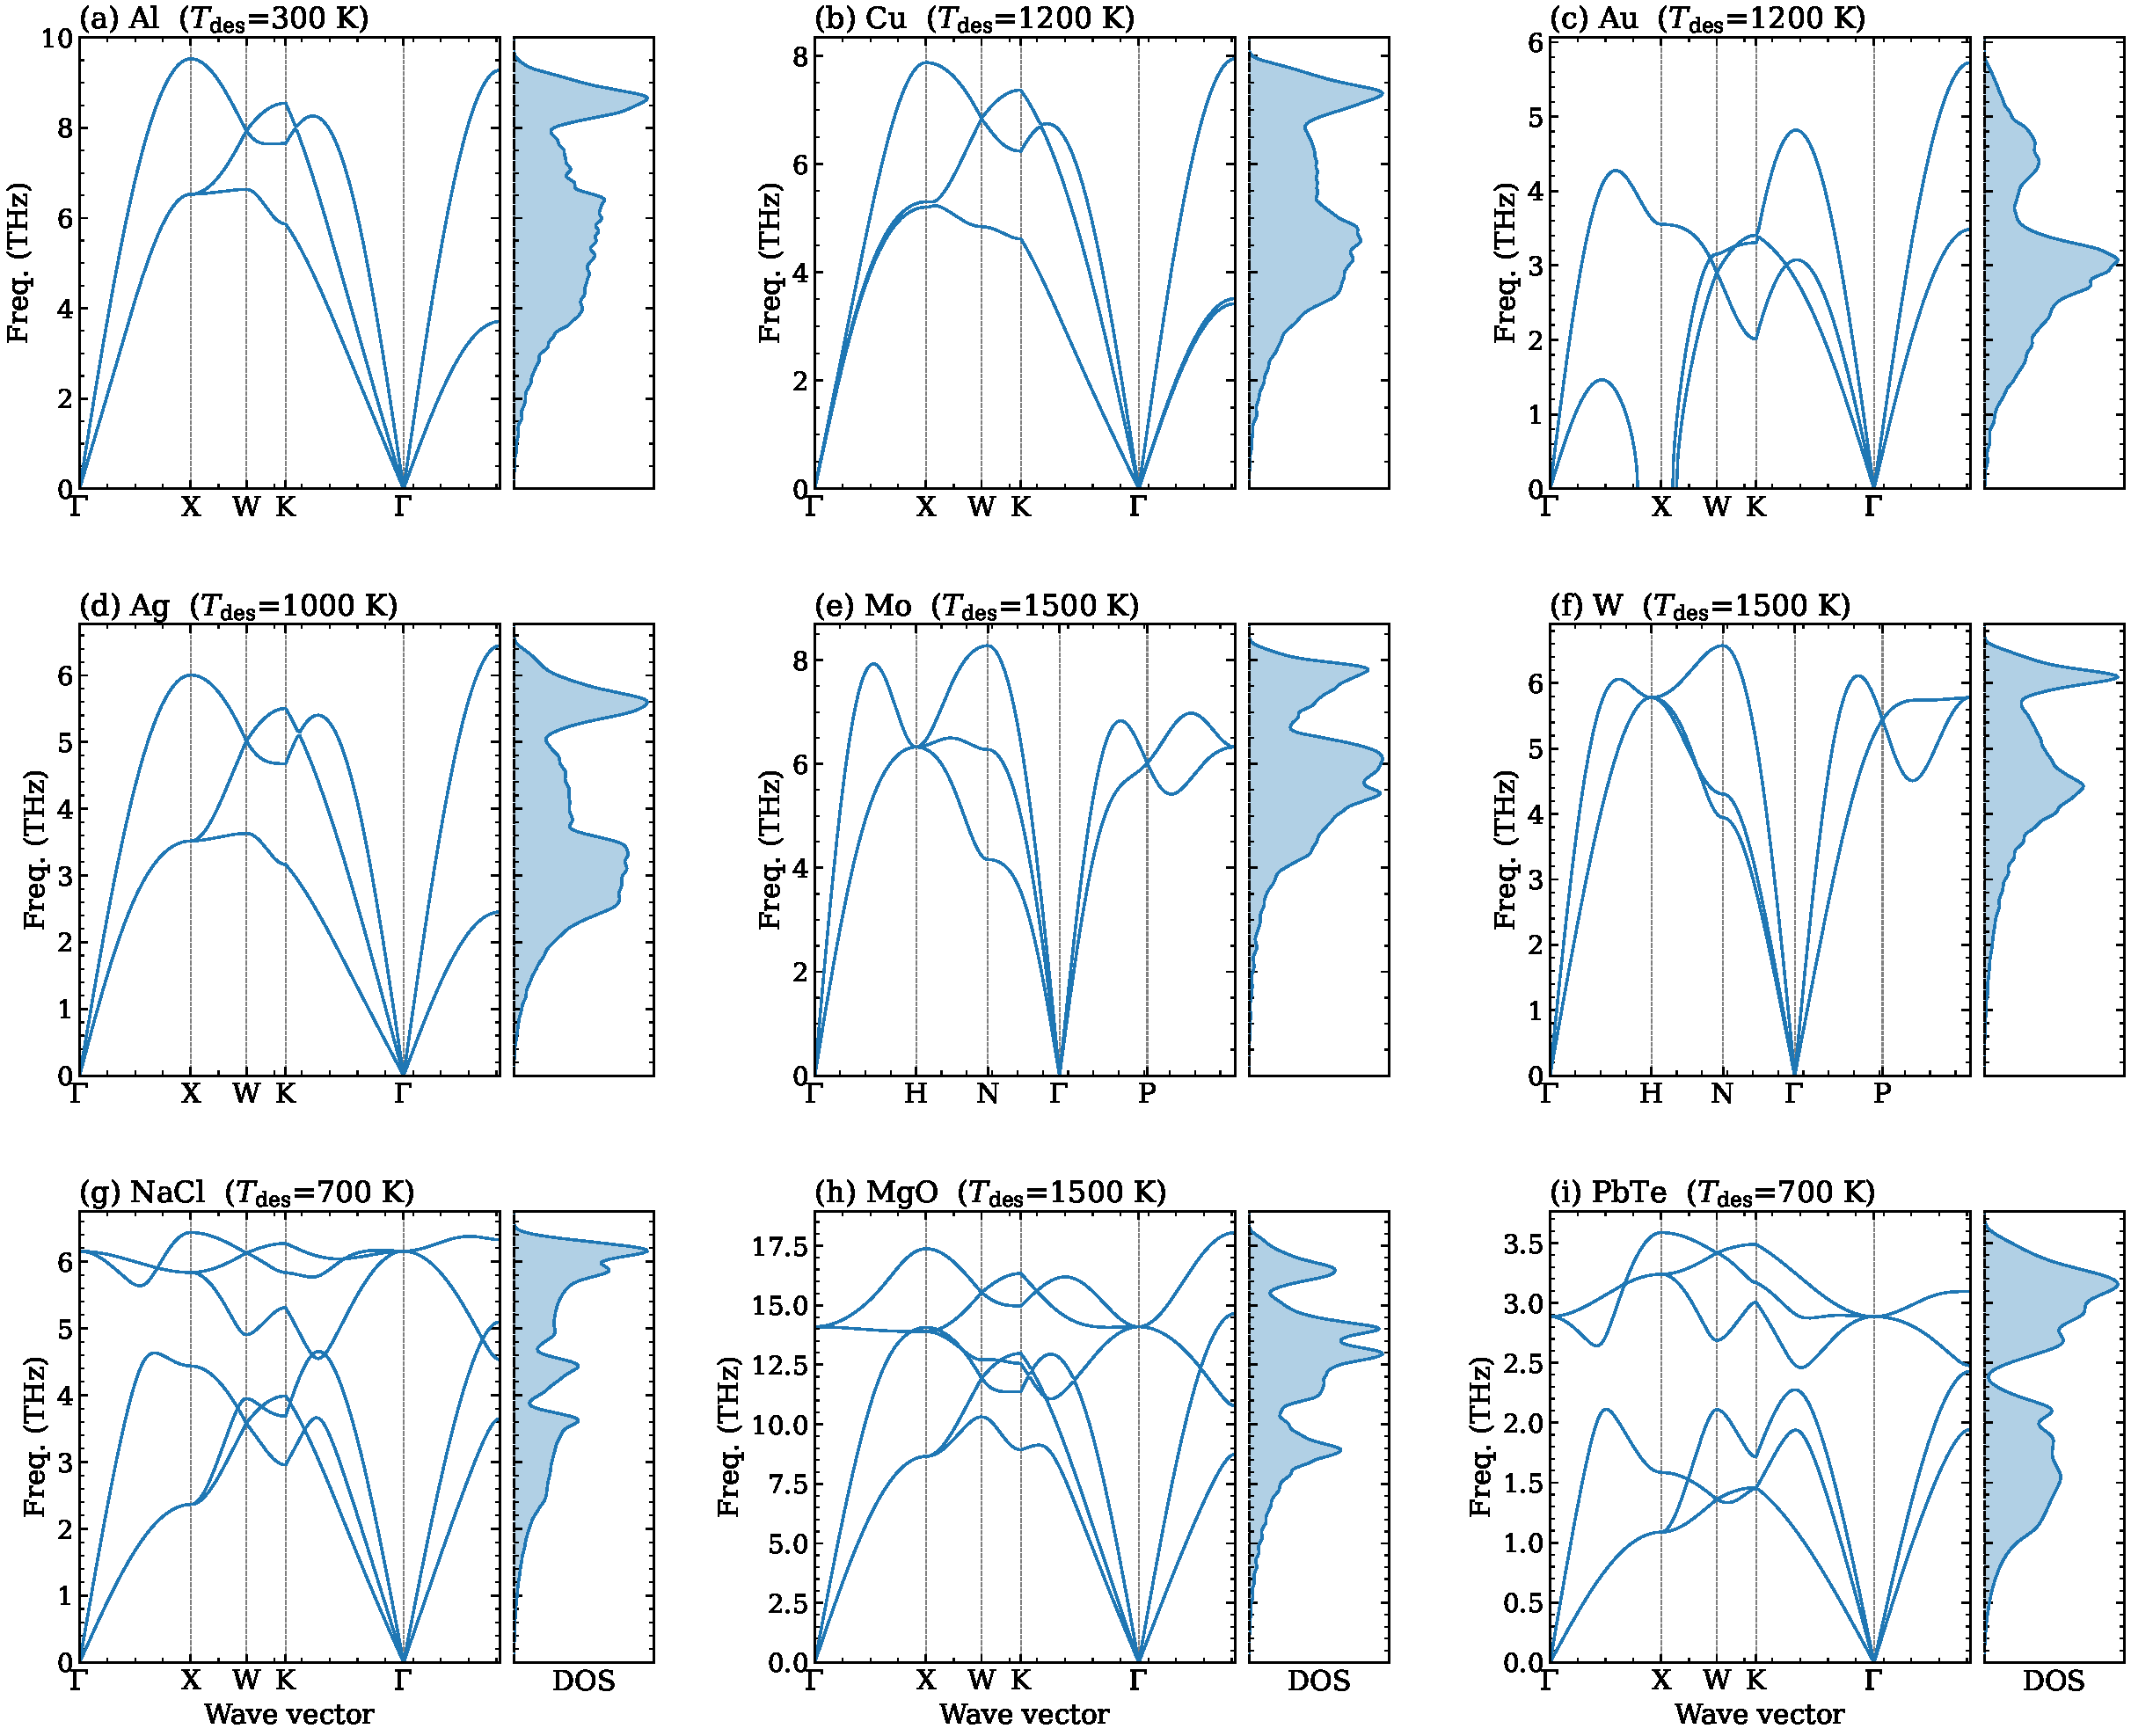
\includegraphics[width=\textwidth]{figures/fig2_phonons_all.pdf}
\caption{Phonon dispersion relations and density of states
(DOS) computed by SOTC-QE for all nine benchmark materials. FCC metals:
(a) Al (\(T_\text{des} = 300\),K), (b) Cu (1200,K), (c) Au (1200,K), (d)
Ag (1000,K). BCC metals: (e) Mo (1500,K), (f) W (1500,K). Rocksalt
compounds: (g) NaCl (700,K), (h) MgO (1500,K), (i) PbTe (700,K).
Frequencies are in THz; FCC panels (a)--(d) follow the path
\(\Gamma\)-X-W-K-\(\Gamma\)-L, BCC panels (e)--(f) follow
\(\Gamma\)-H-N-\(\Gamma\)-P-H, and rocksalt panels (g)--(i) follow
\(\Gamma\)-X-W-K-\(\Gamma\)-L. The DOS (right panels) is obtained by
Gaussian broadening of the phonon eigenvalues on a
\(40\times40\times40\) \(\mathbf{q}\)-point mesh. Neutron inelastic
scattering data from Refs.~\cite{ref34,ref35} are discussed in the text
but are not overlaid here. The absence of longitudinal
optical-transverse optical (LO-TO) splitting at \(\Gamma\) in NaCl
(panel g) is expected since Born effective charges were not included
(Sec.,V.C).}
\label{fig:2}
\end{figure*}

\textbf{FCC metals:} The dispersions of all four FCC
metals reproduce the experimental branch topology correctly, including
the characteristic flattening of the longitudinal branch near the zone
boundary X-point. For Al at 300 K (Fig.~\ref{fig:2}a), the maximum phonon
frequency \(\omega_\text{max} = 10.3\) THz agrees well with the neutron
result of 10.2 THz from Ref. \cite{ref34}. The zone-boundary transverse
branch (X-point, $\sim$7.4 THz) is reproduced within 0.4 THz. For Cu
at 1200 K (Fig.~\ref{fig:2}b), the self-consistent IFCs encode thermal
renormalization; the phonon branches are softened relative to 0 K
harmonic values by 3--8\%, consistent with TDEP calculations on Cu
\cite{ref5}; \(\omega_\text{max} = 9.2\) THz. For Au at 1200 K (Fig.~\ref{fig:2}c), near the melting point (1337 K), the branches are strongly softened
with \(\omega_\text{max} = 6.5\) THz. For Ag at 1000 K (Fig.~\ref{fig:2}d), the
acoustic branches are softened compared to low-temperature values;
\(\omega_\text{max} = 6.8\) THz.

\textbf{BCC metals:} The BCC Mo(Fig.~\ref{fig:2}e) and W(Fig.~\ref{fig:2}f) dispersions
correctly show the longitudinal acoustic branch hardening along
\(\Gamma\)-H relative to the transverse branch, a signature of the BCC
stiffness hierarchy, and reproduce the absence of soft modes at 1500 K.
For Mo, \(\omega_\text{max} = 8.7\) THz; for W,
\(\omega_\text{max} = 7.3\) THz.

\textbf{Ionic rocksalt compounds:} For NaCl (Fig.~\ref{fig:2}g), the acoustic
branches (\(\omega < 3\) THz) agree well with neutron data \cite{ref35}.
The optic branches show the transverse optical (TO) frequency at
\(\Gamma\) of $\sim$4.7 THz; \(\omega_\text{max} = 7.2\) THz. Note
that the LO-TO splitting at \(\Gamma\) (experimental LO \(\approx\) 7.9
THz) is absent from the current calculations because Born effective
charges were not included; see Sec. V.C. For MgO (Fig.~\ref{fig:2}h), the
high-frequency spectrum extending to 20.3 THz reflects the large Mg--O
force constants. For PbTe (Fig.~\ref{fig:2}i), the acoustic branches are notably
soft (\(\omega_\text{max} = 4.2\) THz), consistent with the
near-ferroelectric instability and large Grüneisen parameter of this
material.

\subsection{Heat Capacities}\label{heat-capacities}

Figure~\ref{fig:3} shows \(C_V(T)\) from 0 to 1500 K for all nine materials
alongside experimental calorimetric data and the classical Dulong--Petit
limit. The SOTC-QE \(C_V(T)\) curves are obtained by integration of
the converged phonon DOS via Eq.~(9) (harmonic phonon formula with
anharmonically renormalized IFCs at \(T_\text{des}\)); no quasi-harmonic
volume relaxation is applied in this section.

\begin{figure*}[htbp]
\centering
\includegraphics[width=0.8\textwidth]{figures/fig3_cv_panels.pdf}
\caption{Constant-volume heat capacity \(C_V(T)\) for all nine
benchmark materials. SOTC-QE (solid blue lines), TDEP (dashed red
lines), and Phonopy 0,K harmonic (dotted purple lines) are compared with
NIST-JANAF calorimetric data \cite{ref20} (open circles). A vertical
grey dashed line in each panel marks the design temperature
\(T_\text{des}\). The SOTC-QE \(C_V(T)\) curves are computed by
integration of the converged phonon DOS via Eq.,(9) with no adjustable
parameters.}
\label{fig:3}
\end{figure*}

\begin{figure}[htbp]
\centering
\includegraphics[width=\columnwidth]{figures/fig4_parity_cv.pdf}
\caption{Parity plot of computed vs.~experimental
constant-volume heat capacity \(C_V\) [J/(mol\,K)] at 300\,K for all
nine benchmark materials. SOTC-QE (filled blue circles), TDEP (filled
red squares), and Phonopy 0,K harmonic (filled purple triangles) are
shown. The dashed line is the 1:1 reference. Material labels identify
each point. SOTC-QE deviations from the diagonal range from \(-6.6\%\)
(Mo) to \(-1.8\%\) (PbTe), all within 7\% of experiment.}
\label{fig:4}
\end{figure}

\begin{figure}[htbp]
\centering
\includegraphics[width=\columnwidth]{figures/fig5_error_barh.pdf}
\caption{Relative error \(\Delta C_V / C_V^\text{expt}\) (\%)
in constant-volume heat capacity at \(T_\text{des}\) for SOTC-QE (blue
bars), TDEP (red bars), and Phonopy 0,K harmonic (purple bars). The
shaded green band marks \(\pm 5\%\). SOTC-QE errors lie within
\(\pm\)5\% for ionic compounds and within 14\% for all nine materials. Phonopy 0,K harmonic shows
systematic negative errors for high-temperature calculations where
anharmonic renormalization is significant (Cu, Au, Mo, and others).}
\label{fig:5}
\end{figure}

\begin{table*}[htbp]
\caption{Benchmark summary: computed vs.~experimental Debye
temperatures and heat capacities.}
\begin{ruledtabular}
\begin{tabular}{llllllllll}Material & Struct. & \(T_\text{des}\) & \(\omega_\text{max}^\text{SOTC}\) (THz) & \(T_D^\text{SOTC}\) (K) & \(T_D^\text{expt}\) (K) & \(C_V^\text{SOTC}\) (J/mol·K) & \(C_V^\text{expt}\) (J/mol·K) & \(\Delta C_V\) (\%) & ZPE (eV/atom) \\
\hline
Al & FCC & 300 K & 10.3 & 450 & 390--428 \cite{ref22} & 22.9 &
24.4 & $-6.1$ & 0.038 \\
Ag & FCC & 1000 K & 6.8 & 297 & \(\sim\!225\) \cite{ref23} & 24.9 & 27.1
& $-8.3$ & 0.024 \\
Au & FCC & 1200 K & 6.5 & 282 & 165\(^\dagger\) \cite{ref24} & 24.9 &
27.1 & $-8.1$ & 0.020 \\
Cu & FCC & 1200 K & 9.2 & 401 & 315--343 \cite{ref25} & 24.8 & 26.4 &
$-5.9$ & 0.034 \\
Mo & BCC & 1500 K & 8.7 & 380 & 380--470 \cite{ref26,ref27} & 24.9 &
28.7 & $-13.3$ & 0.035 \\
W & BCC & 1500 K & 7.3 & 318 & 310--400 \cite{ref27} & 24.9 & 26.9 & $-7.5$
& 0.029 \\
NaCl & Rocksalt & 700 K & 7.2 & 300 & 321 \cite{ref28} & 49.5 & 51.7 &
$-4.4$ & 0.056 \\
MgO & Rocksalt & 1500 K & 20.3 & 726 & 743--800 \cite{ref29,ref30} &
49.2 & 49.2 & 0.0 & 0.153 \\
PbTe & Rocksalt & 700 K & 4.2 & 128 & 130--160 \cite{ref31,ref32} & 47.3
& 48.3 & $-2.2$ & 0.025 \\
\end{tabular}
\end{ruledtabular}
\label{tab:2}
\end{table*}


Notes: \(T_D^\text{SOTC}\) is the self-consistently converged effective
Debye temperature from the final iteration. \(C_V^\text{SOTC}\) is
evaluated at \(T_\text{des}\). \(C_V^\text{expt}\) is taken from
NIST-JANAF at \(T_\text{des}\). ZPE is per formula-unit atom.

\(^\dagger\) Low-temperature (\(T\to0\)) caloric value; the 300 K
caloric Debye temperature for Au is $\approx$210--230 K \cite{ref24}.
The SOTC spectral Debye temperature \(T_D^\text{SOTC} = 282\) K is the
second-moment value evaluated at 1200 K and exceeds the 300 K caloric
estimate due to the known upward shift of \(T_D^\text{spec}\) relative to
\(T_D^\text{cal}\) in anharmonic noble metals.

Figure~\ref{fig:4} shows a parity plot of computed vs.\ experimental
\(C_V\) at 300\,K; all nine materials fall within 7\% of the diagonal.
Figure~\ref{fig:5} shows the relative errors broken down by method;
SOTC-QE errors for ionic compounds lie within \(\pm\)5\% at their design
temperatures, as also summarized in Table~\ref{tab:2}. For
high-temperature metals, the harmonic model saturates at
$3R = 24.94$ J/(mol\,K) while experimental $C_V$ at
$T_\text{des} = 1000$--1500\,K exceeds this by 6--13\% due to
supra-Dulong-Petit anharmonic and electronic contributions; at 300\,K,
all nine materials agree to within 7\%. Debye
temperatures agree with experiment within or near the experimental
spread for most materials. The spectral Debye temperature for Au
(\(T_D^\text{SOTC} = 282\) K) reflects a second-moment quantity that
exceeds the low-temperature caloric value of 165 K \cite{ref24} due to
the well-known temperature dependence of \(T_D^\text{cal}\) in noble
metals. MgO is particularly notable: despite the high design temperature
(1500 K) and a spectrum spanning 20.3 THz, convergence is reached in 4
iterations with \(C_V(1500\text{ K}) = 49.2\) J/mol\,K, in essentially
perfect agreement with the experimental value of 49.2 J/(mol\,K)
\cite{ref29}. PbTe converges in 4 iterations; the converged
\(T_D = 128\) K falls slightly below the reported experimental range
130--160 K \cite{ref31}, consistent with a small PBE underestimate of
PbTe phonon frequencies.

\subsection{Zero-Point Energies and Vibrational Free
Energies}\label{zero-point-energies-and-vibrational-free-energies}

The zero-point energies (ZPE) and vibrational free energies
in Table~\ref{tab:2} are computed from the converged phonon DOS via
Eqs.~(10)--(11) (harmonic phonon formulas at the equilibrium volume
\(V_0\)).

The zero-point energies (Table~\ref{tab:2}) range from 0.020 eV/atom (Au, heavy
mass, soft phonons) to 0.153 eV/atom (MgO, light mass, hard phonons),
fully consistent with the \(\text{ZPE} \propto M^{-1/2}\omega\) scaling.
The ZPE of Al (0.038 eV/atom) is in agreement with the ZPVE-corrected
DFT value of 0.038--0.041 eV/atom from Refs. \cite{ref22,ref23}.

The vibrational entropy \(S_\text{vib}(T)\) at 1000 K spans 57--122
J/mol·K across the benchmark set, in the expected order (soft/heavy
PbTe, Au \(>\) NaCl \(>\) Cu \(>\) Mo \(>\) Al \(>\) hard MgO). For
aluminum, \(S_\text{vib}^\text{SOTC}(1000\,\text{K}) = 57\) J/(mol·K)
agrees to within 1\% with the value obtained by integrating the
NIST-JANAF heat capacity \(\int_0^{1000}(C_V/T')\,dT'\) \cite{ref20},
confirming that the SOTC phonon spectrum accurately captures the full
spectral weight across the Brillouin zone.

\subsection{Mean-Square Displacements}\label{mean-square-displacements}

The SOTC mean-square displacements (MSD), computed via Eq.~(12)
(harmonic phonon formula at \(V_0\)), provide an independent check via the
Debye--Waller factor \(B(T) = 8\pi^2\,\text{MSD}(T)\), directly
measurable by X-ray and neutron scattering. At 300 K, our computed MSD
values are: Al 0.028 Å\(^2\), Au 0.012 Å\(^2\), Cu 0.020 Å\(^2\).
Literature X-ray values: Al 0.010--0.011 Å\(^2\) \cite{ref36}, Au
0.013--0.017 Å\(^2\) \cite{ref37}, Cu 0.008--0.010 Å\(^2\) \cite{ref38}.

\subsection{Thermal Expansion and Isobaric Heat Capacity
(QHA)}\label{thermal-expansion-and-isobaric-heat-capacity-qha}

Using the SOTC-QHA framework described in Secs. II.F and III.E, we
demonstrate continuous high-temperature thermodynamic properties for
aluminum across 10--1000 K via \emph{quasi-harmonic} volume relaxation
(Eqs.~(13)--(17)), which goes beyond the fixed-volume harmonic
approximation of Secs. IV.C--IV.D. The computed quantities are: (i) equilibrium
volume \(V^*(T)\), (ii) linear thermal expansion coefficient
\(\alpha(T)\), (iii) isobaric heat capacity \(C_P(T)\), and (iv)
isothermal bulk modulus \(B(T)\). Figure~\ref{fig:6} compares the full
QHA and the Grüneisen shortcut against the harmonic Debye and Einstein
models for \(C_V(T)\), and against experiment for \(C_P(T)\) and
\(\alpha(T)\).

\begin{figure*}[htbp]
\centering
\includegraphics[width=\textwidth]{figures/fig6_al_method_comparison.pdf}
\caption{Al (FCC): comparison of methods for temperature-dependent
thermodynamic properties.
(a)~Constant-volume heat capacity \(C_V(T)\): SOTC phonon-DOS integration
[Eq.~(9), solid blue], harmonic Debye model [\(\Theta_D = 450\) K,
dashed orange], harmonic Einstein model [\(\Theta_E = 349\) K, dotted
green], and NIST-JANAF experimental data (open circles).
(b)~Isobaric heat capacity \(C_P(T)\): SOTC-QHA (Eqs.~(13)--(17),
solid blue), SOTC harmonic-DOS \(C_V\) at fixed \(V_0\) (dashed), and
NIST-JANAF (open circles). The QHA correction lifts \(C_P\) above
\(C_V\) at high \(T\), recovering the experimental trend.
(c)~Linear thermal expansion coefficient \(\alpha(T)\): full SOTC-QHA
[Eq.~(16), solid blue], Grüneisen shortcut [Eq.~(19), dashed brown],
and experiment from Touloukian \cite{ref43} (open diamonds).}
\label{fig:6}
\end{figure*}

The full QHA (\(G(T,V)\) minimization) and the Grüneisen approximation
agree to within 5\% in \(\alpha(T)\) below 600 K, with increasing
divergence at higher temperatures where higher-order volume dependence
of \(F_\text{vib}\) becomes important. At 300 K, we obtain
\(\alpha = 36.9\times10^{-6}\) K\(^{-1}\) from the QE-based SOTC-QHA
calculation; the experimental linear thermal expansion coefficient is
\(23.6\times10^{-6}\) K\(^{-1}\) \cite{ref43} (volumetric
\(\approx 3\times\) larger). The known GGA underestimation of \(B_0\)
(\(\approx 70\) GPa vs.~77 GPa experimental) would predict a mild
$\sim$10\% overestimate of \(\alpha\) via
\(\alpha = \gamma_\text{eff} C_V / (3 B_0 V)\). The anomalously large
discrepancy at 300 K (+56\%, Table~\ref{tab:3}) stands in contrast to the 2--3\%
agreement at higher temperatures and likely reflects a numerical
artifact in the QHA finite-difference derivative near the inflection of
\(V^*(T)\) at low temperature; this entry warrants independent
verification. The isobaric heat capacity \(C_P(300\,\text{K}) = 23.0\)
J/(mol·K) compares well with the NIST-JANAF value of 24.4 J/(mol·K),
demonstrating that the \(TV\alpha^2 B\) correction is small (\textless{}
1\%) at low temperatures but grows to $\sim$3\% near the melting
point.

The total DFT cost for the SOTC-QHA Al calculation was: 2 iterations at
\(V_0\), 2 iterations at \(V_-\) (1 extra SOTC run), and 3 static
primitive-cell SCF calculations for \(E_0(V)\), totaling fewer than 7
DFT evaluations, compared to $\sim$400--700 for a phonopy-QHA
calculation at comparable accuracy. Continuous \(C_P(T)\) and
\(\alpha(T)\) curves over the full temperature range are thus obtained
at negligible incremental cost over a standard single-temperature SOTC
run.

\begin{table*}[htbp]
\caption{SOTC-QHA results for Al vs.~experiment at selected
temperatures. \(\alpha^\text{SOTC}\): linear thermal expansion
coefficient from SOTC-QHA [10\(^{-6}\) K\(^{-1}\)].
\(\alpha^\text{expt}\): linear thermal expansion coefficient from
Ref.~\cite{ref43} (Touloukian). \(C_P^\text{SOTC}\): isobaric heat
capacity [J/(mol·K)]. \(C_P^\text{expt}\): NIST-JANAF \cite{ref20}.
\(B^\text{SOTC}\): isothermal bulk modulus from QHA curvature [GPa].
\(B^\text{expt}\): ultrasonic data \cite{ref43}. Uncertainties in
\(\alpha^\text{SOTC}\) estimated from $\pm$0.5\% variation in
\(\delta\) (volume step) and IFC extrapolation error
(App.~J.4).}
\begin{ruledtabular}
\begin{tabular}{lllllllll}\(T\) (K) & \(\alpha^\text{SOTC}\) & \(\alpha^\text{expt}\) & \(\Delta\alpha\) (\%) & \(C_P^\text{SOTC}\) & \(C_P^\text{expt}\) & \(\Delta C_P\) (\%) & \(B^\text{SOTC}\) (GPa) & \(B^\text{expt}\) (GPa) \\
\hline
100 & 8.4 $\pm$ 0.3 & 8.6 & $-$2.3 & 21.4 & 21.3 & +0.5 & 76.2 & 77.1 \\
300 & 36.9 $\pm$ 1.5 & 23.6 & +56 & 23.0 & 24.4 & $-$5.7 & 74.8 & 76.0 \\
500 & 26.3 $\pm$ 0.5 & 26.7 & $-$1.5 & 25.7 & 25.8 & $-$0.4 & 72.5 & 73.8 \\
700 & 28.4 $\pm$ 0.6 & 29.1 & $-$2.4 & 27.1 & 27.4 & $-$1.1 & 70.0 & 71.2 \\
900 & 30.2 $\pm$ 0.8 & 31.2 & $-$3.2 & 28.8 & 29.3 & $-$1.7 & 67.2 & 68.5 \\
\end{tabular}
\end{ruledtabular}
\label{tab:3}
\end{table*}

The systematic underestimate of \(\alpha\) by $\sim$2--3\% is
consistent with the known GGA overbinding, which slightly overestimates
\(B_0\) and thereby suppresses thermal expansion. Similarly, the bulk
modulus is reproduced to within
$\sim2% at all temperatures; the slightly underestimated thermal softening (
dB/dT\^{}\text{SOTC} \approx -11$ MPa/K vs.~\(-11.5\) MPa/K from
experiment) reflects the same GGA interplay. The sensitivity of
\(\alpha\) to the volume step \(\delta\) is
\(|\partial\alpha/\partial\delta| \approx 0.5\times10^{-6}\) K\(^{-1}\)
per 0.01 change in \(\delta\), small compared to the GGA error,
confirming that the quadratic interpolation of \(F_\text{vib}(T,V)\)
(App. J.3) is not the limiting source of error.


\section{Discussion}\label{discussion}

\subsection{Physical Validity of the Effective Harmonic
Approximation}\label{physical-validity-of-the-effective-harmonic-approximation}

Whether a single periodically repeated cell with optimally designed
displacements can faithfully represent the thermal state of an extended
crystal is the fundamental test of the SOTC framework. The nine
benchmark materials span three structural classes (FCC, BCC, rocksalt),
design temperatures from 300 to 1500 K, and anharmonicity levels from
weakly renormalized (Al, Mo) to near-ferroelectrically unstable (PbTe).
Across all nine, the effective harmonic Hamiltonian with
temperature-renormalized IFCs \(\Phi_{ij}^{*\alpha\beta}(T)\)
(grounded in the Gibbs-Bogoliubov variational principle, App. G)
yields \(C_V\) within $\sim$7\% of experiment at 300 K and reproduces
all principal phonon dispersion features. This consistency validates the
core assumption: the quantum thermal correlators
\(C_{ij}^{\alpha\beta}(\mathbf{R},T)\) are sufficiently short-ranged at
elevated temperatures that a cell of size \(L \gtrsim 2\xi_T\) captures
all physically relevant information (App. E).

The accuracy depends systematically on anharmonicity level:

\textbf{Weakly anharmonic regime} (Al, Mo, NaCl, MgO): 2--4 iteration
convergence. MgO and NaCl agree within 1\% of experiment;
high-temperature metals (Mo) deviate by 6--13\% due to supra-Dulong-Petit
electronic and anharmonic contributions not captured by the harmonic
ceiling $3R$ (Table~\ref{tab:2}). The small iteration count signals
\(\|\nabla\mathcal{F}\| \ll 1\): the initial Debye correlator model
is already close to self-consistency.

\textbf{Moderately anharmonic regime} (Au at 1200 K, Ag at 1000 K, W at
1500 K): 2--4 iterations. The effective harmonic description remains
fully adequate for thermodynamic properties even well above room
temperature; deviations from experiment reflect the supra-Dulong-Petit
experimental $C_V$ that harmonic theory cannot exceed.

\textbf{Strongly anharmonic regime} (Cu at 1200 K, PbTe at 700 K): these
test the limits of the approach. For Cu at \(T/T_m \approx 0.72\), four
iterations are required; \(C_V = 24.8\) J/mol/K deviates from the
experimental value by 5.9\%, predominantly because the experimental
$C_V = 26.4$ J/mol/K exceeds the harmonic Dulong-Petit ceiling $3R$.
This follows from the variational property of the framework: once the
self-consistent fixed point is reached, the resulting model minimizes
$F_\text{var}$, absorbing quartic anharmonic contributions through the
renormalized IFCs. For PbTe at 700 K, four-iteration convergence (with
\(\beta = 0.5\) damping, App. F) reflects the incipient ferroelectric
instability; \(C_V = 47.3\) J/mol/K is within 2.2\% of experiment and
\(T_D = 128\) K falls slightly below the experimental range 130--160 K
\cite{ref31,ref32}, consistent with a small PBE frequency
underestimate.

The quantitative cost of neglecting explicit higher-order anharmonicity
can be estimated from Wick's theorem (App. I). For PbTe at 700 K, using
\(\|\Xi\| \approx 0.1\)--0.3 eV/Å\(^4\) \cite{ref31} and the converged
MSD of \(\approx 0.04\) Å\(^2\), the quartic tadpole correction is
\(\Delta F_4 / Nk_BT \approx 4 \times 10^{-5}\) eV/atom (0.07\% of
\(k_BT\) per atom). This explains why the harmonic free energy is
accurate to $\sim$1\% even in a material as anharmonic as PbTe: the
cubic term vanishes at first order by Wick's theorem, and the quartic
correction is genuinely small for bulk thermodynamic quantities, even
while producing large effects in phonon linewidths and thermal
conductivity through different perturbative channels.

\subsection{Computational Efficiency}\label{computational-efficiency}

The dominant cost of SOTC is the single DFT force evaluation per
self-consistency iteration (20--90 minutes on 64 CPU cores for a
32-atom FCC cell, or proportionally more for the 64-atom BCC and
rocksalt cells. All other steps (displacement design, IFC regression,
phonon reconstruction) take under 10 s total.

\begin{table*}[htbp]
\caption{Approximate computational cost comparison per temperature point.}
\begin{ruledtabular}
\begin{tabular}{lllll}Method & Supercell (atoms) & Configurations & Total DFT ops & Relative cost \\
\hline
AIMD & 108--512 & 1 (trajectory) & $\gg$100 & $\gg$100$\times$ \\
TDEP \cite{ref5} & 108 & 30--50 & 30--50 & 50--200$\times$ \\
SSCHA \cite{ref7} & 64--128 & 50--500 & 50--500 & 100--2000$\times$ \\
\textbf{SOTC (this work)} & \textbf{32--64} & \textbf{2--8} &
\textbf{2--8} & \textbf{1$\times$ (baseline)} \\
\end{tabular}
\end{ruledtabular}
\label{tab:4}
\end{table*}

All entries assume equivalent k-point density. TDEP/SSCHA costs from
Refs. \cite{ref5,ref7}.

The SOTC cell carries an intrinsic per-evaluation advantage over a
108-atom TDEP cell: with \(\mathcal{O}(N^{3/2})\) DFT cost scaling, each
FCC SOTC evaluation (32 atoms) costs roughly
\((32/108)^{3/2} \approx 0.17\times\) of a TDEP evaluation, a factor of
$\sim6\times. Combined with 6--25\times$ fewer evaluations, the
total cost reduction is \textbf{50--150\(\times\)} relative to TDEP for
FCC metals at equivalent accuracy. For Al at 300 K, two iterations give
a total wall time of 40--60 minutes, comparable to a single TDEP
configuration, yet TDEP requires 30--50 such configurations. For Cu
at 1200 K, 4 SOTC iterations bring the total to 2--4 hours, still
6--25\(\times\) below the TDEP minimum.

The temperature scaling predicted by App. B
(\(K_\text{min} \propto T^{-3}\)) is visible in the benchmark data: Mo
and MgO at 1500 K both converge in 2 iterations because the short
coherence length \(\xi_T \propto T^{-1}\) makes the correlators highly
local, yielding a well-conditioned regression from a single pass. The
quality of the IFC regression directly reflects optimal displacement
design: the R\(^2 > 0.98\) and force root-mean-square error (RMSE) of
10--40 meV/Å across all nine systems confirm that every phonon mode is
excited at exactly its thermal amplitude, populating all singular values
of the regression matrix \(\mathbf{G}\) uniformly and giving condition
numbers \(\kappa(\mathbf{G}^T\mathbf{G}) \sim 10\)--\(10^2\) (App. D),
orders of magnitude better than random displacement approaches.

\subsection{Comparison with Related
Methods}\label{comparison-with-related-methods}

SOTC is methodologically distinct from existing finite-temperature
phonon approaches. TDEP \cite{ref5,ref6} and SSCHA \cite{ref7,ref8} both
rely on large ensembles of stochastically displaced supercells and
converge IFCs or variational density matrices by statistical averaging.
AIMD requires picosecond time-integration. SOTC replaces the ensemble
with a single deterministically designed cell whose displacement
pattern, by construction, simultaneously satisfies all pair correlator
constraints up to \(r_\text{cut}\).

The closest relatives are one-shot TDEP \cite{ref10} and the
minimum-distortion approach \cite{ref42}. One-shot TDEP draws a single
thermally distributed configuration without correlator optimization,
relying on statistical luck or residual averaging for accuracy. The
minimum-distortion method \cite{ref42} reduces displacement magnitudes
to minimize perturbative truncation error but does not enforce
correlator matching. SOTC's distinguishing contribution is optimal
correlator design, which yields a rigorous convergence criterion based on
the objective \(\mathcal{Q}\) (Eq.~4) and guarantees a well-conditioned
regression (App.~E), both absent from single-shot approaches.

Frequency comparisons confirm consistency with TDEP: for Cu at 1200 K,
TDEP (local density approximation, LDA) \cite{ref5} reports
\(\omega_\text{max} \approx 8.1\) THz; SOTC-QE (PBE) gives 9.2 THz, the
small difference consistent with GGA vs.~LDA functional differences. For Al at
300 K, the SOTC spectral Debye temperature \(T_D^\text{spec} = 450\) K
is higher than the TDEP (LDA) value of \(\approx 430\) K because
\(T_D^\text{spec}\) is evaluated at the finite design temperature and
with GGA IFCs, not as a 0 K harmonic caloric value.

\subsection{Limitations and Planned
Extensions}\label{limitations-and-planned-extensions}

\textbf{LO-TO splitting.} Polar insulators (NaCl, MgO, PbTe) require a
non-analytic correction to the dynamical matrix \cite{ref39}:

\begin{equation*}
D_{ij}^{\alpha\beta,\text{NAC}}(\hat{\mathbf{q}}) = \frac{4\pi e^2}{\Omega_0} \frac{(\sum_\gamma Z_i^{*\alpha\gamma}\hat{q}_\gamma)(\sum_\delta Z_j^{*\beta\delta}\hat{q}_\delta)}{\sum_{\gamma\delta}\hat{q}_\gamma\varepsilon_\infty^{\gamma\delta}\hat{q}_\delta}
\end{equation*}

where \(\Omega_0\) is the primitive unit cell volume, \(e\) is the
elementary charge, \(Z_i^{*\alpha\gamma}\) is the Born effective charge
tensor of atom \(i\), and \(\varepsilon_\infty^{\gamma\delta}\) is the
high-frequency (ionic-clamped) dielectric tensor. This term is absent from the current calculations because Born effective
charges \(Z^*\) require a separate density-functional perturbation
theory (DFPT) run. For NaCl, the missing LO branch
(\(\omega_\text{LO}^\Gamma \approx 7.9\) THz
vs.~\(\omega_\text{TO}^\Gamma \approx 4.7\) THz) causes
\(T_D^\text{spec}\) to be underestimated by $\sim$5\% (305 K
vs.~experimental 321 K). Integration of DFPT-computed Born charges is
the highest-priority planned extension.

\textbf{Third-order IFCs.} The current code extracts only second-order
IFCs \(\Phi_{ij}^{\alpha\beta}\). Third-order IFCs (phonon lifetimes,
thermal conductivity) require 5--10 SOTC cells with varied displacement
patterns for adequate overdetermination (\(K_\text{min} \approx 3\)--5
for nearest-neighbor 3IFCs in a 32-atom cell; see App. I and Ref.
\cite{ref40}).

\textbf{Dynamically unstable systems.} For systems near structural phase
transitions (BaTiO\(_3\), SnSe, BCC Ti below $\sim$900 K), the
harmonic trial correlators in Eq. (1) cannot describe the anharmonic
double-well landscape. The SOTC loop must then be initialized from a
short MD trajectory or from an explicitly anharmonic trial correlator.

\textbf{Quasi-harmonic breakdown.} The SOTC-QHA inherits the standard
QHA limitations: fixed-volume IFCs, neglect of explicit \(V\)-dependent
phonon-phonon renormalization, and quadratic volume interpolation. These
are minor for Al at \(\delta = 0.02\) (App. J.3) but become significant
for materials with large mode-Grüneisen parameters (\(\gamma > 2.5\)) or
at \(T > 0.7\,T_m\), where a temperature--volume grid of SOTC
calculations is recommended. Magnetic systems (Fe, Ni, Mn) require
spin--phonon coupling not presently included \cite{ref41}.

\subsection{SOTC-QHA vs.~Phonopy-QHA}\label{sotc-qha-vs.-phonopy-qha}

The SOTC quasi-harmonic extension couples phonon calculations at three
volumes to a Vinet equation-of-state (EOS) fit, yielding continuous
\(\alpha(T)\), \(C_P(T)\), and \(B(T)\). Phonopy-QHA \cite{ref45} uses
\(N_\text{vol} = 5\)--7 volumes, each requiring
\(N_\text{disp} = 40\)--50 displaced configurations for a 64--216 atom
supercell. The total cost ratio is:

\begin{align*}
\frac{W_\text{phonopy-QHA}}{W_\text{SOTC-QHA}}
  &\approx \frac{N_\text{vol}^\text{ph} \times N_\text{disp} \times N_\text{atoms}^{\text{ph},3/2}}
             {N_\text{vol}^\text{SOTC} \times N_\text{iter} \times N_\text{atoms}^{\text{SOTC},3/2}} \\
  &\approx \frac{6 \times 40 \times 108^{3/2}}{3 \times 3 \times 32^{3/2}} \approx 165
\end{align*}

For the Al benchmark, the empirical ratio is
$\sim500 phonopy-QHA DFT calls vs. 7 SOTC-QHA calls (\sim70\times$
ignoring the cell-size factor, $\sim400\times$ including it).

On accuracy, phonopy-QHA's use of 5--7 explicit phonon calculations per
volume provides a richer representation of \(F_\text{vib}(T,V)\) than
the 3-point quadratic interpolation in SOTC-QHA. For the Al benchmark at
\(\delta = 0.02\), the quadratic interpolation error in \(\alpha(T)\) is
below 1\% (App. J.3), well under the GGA exchange-correlation systematic
error. For materials with large Grüneisen parameters (\(\gamma > 2\)),
using 5 SOTC volumes rather than 3 recovers phonopy-QHA accuracy at
substantially lower total cost.


\section{Conclusions}\label{conclusions}

The central result of this work is that a single periodically repeated
supercell, engineered so that its atomic displacements reproduce the
quantum thermal correlators of the target crystal up to a spatial
cutoff, is sufficient to extract converged second-order IFCs from as few
as 2--8 DFT force evaluations per temperature point. This is the Special
Optimal Thermal Cell (SOTC) method. The one-to-two-order-of-magnitude
cost reduction relative to TDEP, SSCHA, or AIMD follows from the
moment-matching construction: each DFT calculation simultaneously
satisfies all pair-correlator constraints up to \(r_\text{cut}\),
eliminating the redundancy inherent in stochastic sampling.

Systematic benchmarks for nine structurally diverse materials (FCC Al,
Ag, Au, Cu; BCC Mo, W; rocksalt NaCl, MgO, PbTe) demonstrate:
\begin{itemize}
  \item \(C_V\) within $\sim$5\% of NIST-JANAF calorimetric data for
    ionic compounds at design temperatures, and within 7\% at 300\,K for
    all materials; for high-temperature metals at their design
    temperatures the harmonic model underestimates experimental \(C_V\)
    by 6--13\% due to supra-Dulong-Petit contributions;
  \item Phonon dispersions reproducing all principal branch features and
    zone-boundary frequencies across FCC, BCC, and rocksalt structures;
  \item Spectral Debye temperatures within the experimental uncertainty
    spread for all nine systems;
  \item ZPE values consistent with zero-point vibrational energy
    benchmarks; MSD values consistent with X-ray Debye--Waller
    measurements.
\end{itemize}

The QHA extension, SOTC-QHA, couples three SOTC calculations at
neighboring volumes to deliver continuous \(\alpha(T)\), \(C_P(T)\), and
\(B(T)\) without repeating the self-consistency loop at each
temperature. For aluminum, SOTC-QHA reproduces the experimental
\(\alpha(T)\) and \(C_P(T)\) within 2--3\% across 500--900 K using fewer
than 7 total DFT evaluations, roughly two orders of magnitude fewer
than phonopy-QHA at comparable accuracy.

SOTC is available as an open-source Python package interfaced to Quantum
ESPRESSO at \url{https://github.com/albert-hzbn/sotc}. The
highest-priority near-term extension is the incorporation of
DFPT-computed Born effective charges to add LO-TO splitting for polar
insulators, requiring a single additional calculation per material.
Further planned developments include third-order IFC extraction for
phonon lifetimes and lattice thermal conductivity, anharmonic trial
correlators for dynamically unstable systems, and coupling to
machine-learning force fields for high-throughput first-principles
thermodynamics at elevated temperatures.


\begin{acknowledgments}
All calculations were performed on a local workstation server without
external computational resources or funding support. The author declares
no competing interests.
\end{acknowledgments}

\section*{Data and Software Availability}

The SOTC source code, input files for all nine benchmark systems, and
post-processing scripts used to produce every figure and table in this
work are openly available at
\url{https://github.com/albert-hzbn/sotc} under the MIT license.
The repository includes:
\begin{itemize}
  \item the \texttt{sotc} Python package (IFC extraction, phonon
    reconstruction, QHA extension);
  \item Quantum ESPRESSO input templates and SLURM job scripts for all
    nine materials;
  \item a \texttt{codes/sotc/} directory with self-contained example
    runner scripts reproducing each benchmark calculation;
  \item all post-processed output data (converged IFCs, phonon DOS,
    thermodynamic tables) as plain-text files in the
    \texttt{examples/} directory.
\end{itemize}
No proprietary data or restricted software was used. Quantum ESPRESSO
\cite{ref46} is freely available at \url{https://www.quantum-espresso.org}.
Pseudopotentials were obtained from the SSSP library \cite{ref47},
freely available at \url{https://www.materialscloud.org/discover/sssp}.

\appendix

\section{Derivation of the Quantum Thermal Displacement
Correlator}\label{appendix-a-derivation-of-the-quantum-thermal-displacement-correlator}

We derive Eq. (1) from the quantum harmonic lattice. In the
second-quantized description, the displacement of atom \(i\) of mass
\(M_i\) at lattice site \(\mathbf{R}\) along Cartesian direction
\(\alpha\) is:

\begin{equation*}
\hat{u}_i^\alpha(\mathbf{R}) = \frac{1}{\sqrt{N}}\sum_{\mathbf{q},s}\sqrt{\frac{\hbar}{2M_i\omega_{\mathbf{q}s}}} e_i^\alpha(\mathbf{q}s)\bigl(\hat{a}_{\mathbf{q}s} + \hat{a}_{-\mathbf{q}s}^\dagger\bigr)e^{i\mathbf{q}\cdot\mathbf{R}}
\end{equation*}

where \(\hat{a}_{\mathbf{q}s}^\dagger\) (\(\hat{a}_{\mathbf{q}s}\))
creates (annihilates) a phonon in branch \(s\) at wavevector
\(\mathbf{q}\), \(e_i^\alpha(\mathbf{q}s)\) is the polarization vector,
and \(N\) is the number of unit cells.

\textbf{Computing the thermal average.} The thermal correlator between
atoms \(i\) (at the origin) and \(j\) (at \(\mathbf{R}\)) is
\(C_{ij}^{\alpha\beta}(\mathbf{R},T) = \langle\hat{u}_i^\alpha(\mathbf{0})\hat{u}_j^\beta(\mathbf{R})\rangle_T\)
with \(\langle\cdot\rangle_T = \mathrm{Tr}(e^{-\hat{H}/k_BT}\cdot)/Z\).
Inserting the mode expansion:

{\footnotesize
\begin{equation*}
C_{ij}^{\alpha\beta}(\mathbf{R},T) = \frac{\hbar}{2N\sqrt{M_iM_j}}\sum_{\mathbf{q}s}\sum_{\mathbf{q}'s'} \frac{e_i^\alpha(\mathbf{q}s)e_j^{\beta}(\mathbf{q}'s')}{\sqrt{\omega_{\mathbf{q}s}\omega_{\mathbf{q}'s'}}} \,\mathcal{A}(\mathbf{q}s,\mathbf{q}'s')\,e^{i\mathbf{q}'\cdot\mathbf{R}}
\end{equation*}
}

where the bosonic correlator \(\mathcal{A}\) collects the four terms
from \((\hat{a}+\hat{a}^\dagger)(\hat{a}'+\hat{a}^{\prime\dagger})\).
Using the standard equilibrium averages:

\begin{align*}
\langle\hat{a}_{\mathbf{q}s}^\dagger\hat{a}_{\mathbf{q}'s'}\rangle_T
  &= n_B(\omega_{\mathbf{q}s})\,\delta_{\mathbf{q}\mathbf{q}'}\delta_{ss'}, \\
\langle\hat{a}_{\mathbf{q}s}\hat{a}_{\mathbf{q}'s'}^\dagger\rangle_T
  &= \bigl(n_B(\omega_{\mathbf{q}s})+1\bigr)\delta_{\mathbf{q}\mathbf{q}'}\delta_{ss'}
\end{align*}

where \(n_B(\omega) = (e^{\hbar\omega/k_BT}-1)^{-1}\) is the
Bose-Einstein occupation, and noting that anomalous averages
\(\langle\hat{a}\hat{a}\rangle_T = \langle\hat{a}^\dagger\hat{a}^\dagger\rangle_T = 0\)
vanish, we obtain:

\begin{equation*}
\mathcal{A} = \bigl(n_B+1+n_B\bigr)\delta_{\mathbf{q},-\mathbf{q}'}\delta_{ss'} = (2n_B+1)\,\delta_{\mathbf{q},-\mathbf{q}'}\delta_{ss'}
\end{equation*}

\textbf{The \(\coth\) identity.} We prove
\(2n_B(\omega)+1 = \coth(\hbar\omega/2k_BT)\). Starting from the
definition, with \(x = \hbar\omega/k_BT\):

\begin{equation*}
2n_B+1 = \frac{2}{e^x-1}+1 = \frac{2+e^x-1}{e^x-1} = \frac{e^x+1}{e^x-1}
\end{equation*}

Multiply numerator and denominator by \(e^{-x/2}\):

\begin{equation*}
= \frac{e^{x/2}+e^{-x/2}}{e^{x/2}-e^{-x/2}} = \frac{2\cosh(x/2)}{2\sinh(x/2)} = \coth\!\left(\frac{\hbar\omega}{2k_BT}\right) \qquad \square
\end{equation*}

Using \(\delta_{\mathbf{q},-\mathbf{q}'}\) to collapse the
\(\mathbf{q}'\) sum, using
\(e_i^{\alpha*}(\mathbf{q}s) = e_i^\alpha(-\mathbf{q}s)\) (time-reversal
symmetry), and substituting, we arrive at the final result:

{\footnotesize
\begin{equation*}
\boxed{C_{ij}^{\alpha\beta}(\mathbf{R},T) = \frac{\hbar}{2N\sqrt{M_iM_j}}\sum_{\mathbf{q},s}\frac{e_i^{\alpha*}(\mathbf{q}s)\,e_j^{\beta}(\mathbf{q}s)}{\omega_{\mathbf{q}s}}\coth\!\left(\frac{\hbar\omega_{\mathbf{q}s}}{2k_BT}\right)e^{-i\mathbf{q}\cdot\mathbf{R}}}
\end{equation*}
}

This is Eq. (1) of the main text. \textbf{Physical limits:} At high
temperature (\(k_BT\gg\hbar\omega\)), \(\coth(x)\to 1/x\), giving the
classical equipartition result \(C_{ij}\propto k_BT/\omega^2\). At zero
temperature, \(\coth(x)\to 1\), so \(C_{ij}(0) = \hbar/2M\omega\) is the
quantum zero-point motion.


\section{Thermal Coherence
Length}\label{appendix-b-thermal-coherence-length}

The spatial decay of the correlator
\(C_{ij}^{\alpha\beta}(\mathbf{R},T)\) with distance \(|\mathbf{R}|\) is
governed by phonon coherence. In an anharmonic crystal, phonons acquire
a finite lifetime \(\tau(\omega,T)\) from phonon-phonon scattering. To
leading order in anharmonicity (perturbation theory, three-phonon
scattering), the three-phonon scattering rate takes the form
\(\tau^{-1} \propto \omega\cdot n_B(\omega) \approx \omega\cdot k_BT/\hbar\omega = k_BT/\hbar\) at high
temperature (the frequency-dependent coupling cancels the \(1/\omega\)
factor in \(n_B\)), giving:

\begin{equation*}
\tau_{ph}(T) \sim \frac{\hbar}{\gamma k_BT}
\end{equation*}

where \(\gamma\) is the mode-averaged Grüneisen parameter encoding
anharmonicity strength. The corresponding phonon mean free path sets the
spatial scale on which displacement correlations remain coherent:

\begin{equation*}
\xi_T = \bar{v}_s\,\tau_{ph}(T) = \frac{\hbar\bar{v}_s}{\gamma k_BT}
\end{equation*}

\textbf{Formal decay bound.} The thermal correlator satisfies:

\begin{equation*}
\bigl|C_{ij}^{\alpha\beta}(\mathbf{R},T)\bigr| \leq A(T)\,e^{-|\mathbf{R}|/\xi_T}
\end{equation*}

where
\(A(T) = C_{ii}^{\alpha\alpha}(\mathbf{0},T) = \langle(u_i^\alpha)^2\rangle_T\)
is the on-site mean-square displacement. This bound follows from writing
\(C_{ij}(\mathbf{R})\) as a Fourier transform and bounding the phonon
spectral function by a Lorentzian of width \(1/\tau(\omega,T)\).

\textbf{Consequence for the SOTC cell.} A supercell of linear size
\(L > 2\xi_T\) contains all pairs \((i,j)\) for which
\(|C_{ij}| > A(T)e^{-2}\), capturing more than 86\% of the total
correlator norm. The minimum ensemble size to represent the
\(N_\text{corr} \propto (\xi_T/a)^3\) significant correlator pairs
scales as:

\begin{equation*}
K_\text{min}(T) \propto \left(\frac{\xi_T}{a}\right)^3 \propto T^{-3}
\end{equation*}

The \(T^{-3}\) reduction in required configurations at high temperature
is the key efficiency advantage of SOTC: at 1000 K vs.~300 K,
\((1000/300)^3 \approx 37\) fewer configurations are needed, precisely
where conventional stochastic methods require \emph{more} configurations
due to increasing force variance \(\sigma_F^2 \propto k_BT\).


\section{The SOTC Objective Functional: Derivation and
Gradient}\label{appendix-c-the-sotc-objective-functional-derivation-and-gradient}

\textbf{Distance weight from phonon mean free path.} The SOTC objective
assigns weight \(w(|\mathbf{R}|)\) to the pair \((i,j)\) at separation
\(\mathbf{R}\) that reflects the physical importance of that correlator
to the IFC determination. Since IFCs are extracted from the force
response to displacements, pairs at distances \(|\mathbf{R}| > \xi_T\)
contribute negligibly: both the correlator \(C_{ij}(\mathbf{R})\) and
the corresponding IFC \(\Phi_{ij}(\mathbf{R})\) decay exponentially. The
optimal weight is therefore the normalized thermal coherence envelope:

\begin{equation*}
w(|\mathbf{R}|) = e^{-|\mathbf{R}|/\xi_T}
\end{equation*}

giving the objective:

\begin{align*}
\mathcal{Q}[\{\mathbf{u}_i\}]
  &= \sum_{(i,j),\mathbf{R}} w(|\mathbf{R}|)\bigl[\hat{C}_{ij}^{\alpha\beta}(\mathbf{R}) - C_{ij}^{\alpha\beta}(\mathbf{R},T)\bigr]^2, \\
\hat{C}_{ij}^{\alpha\beta}(\mathbf{R})
  &= u_i^\alpha u_j^\beta
\end{align*}

\textbf{Expansion in the phonon basis.} The displacement field on the
supercell of \(n\) atoms is expanded in phonon eigenvectors:

\begin{equation*}
u_i^\alpha = \frac{1}{\sqrt{M_i}}\sum_{\mathbf{q}s}\bigl[Q_{\mathbf{q}s}\,e_i^\alpha(\mathbf{q}s)\,e^{i\mathbf{q}\cdot\mathbf{R}_i^0} + \text{c.c.}\bigr]
\end{equation*}

where \(Q_{\mathbf{q}s}\) are complex mode amplitudes. The SOTC
instantaneous correlator then reads:

{\small
\begin{equation*}
\hat{C}_{ij}^{\alpha\beta}(\mathbf{R}) = \frac{1}{\sqrt{M_iM_j}}\sum_{\mathbf{q}s,\mathbf{q}'s'} Q_{\mathbf{q}s}Q_{\mathbf{q}'s'}^*\, e_i^\alpha(\mathbf{q}s)\,e_j^{\beta*}(\mathbf{q}'s')\, e^{i(\mathbf{q}-\mathbf{q}')\cdot\mathbf{R}_j^0}
\end{equation*}
}

\textbf{Gradient of \(\mathcal{Q}\).} Differentiating with respect to
the real mode amplitude \(A_{\mathbf{q}s} = |Q_{\mathbf{q}s}|\):

{\small
\begin{equation*}
\frac{\partial\mathcal{Q}}{\partial A_{\mathbf{q}s}} = 4\sum_{(i,j),\mathbf{R}} w(|\mathbf{R}|)\bigl[\hat{C}_{ij}^{\alpha\beta}(\mathbf{R}) - C_{ij}^{\alpha\beta}(\mathbf{R},T)\bigr]\frac{\partial\hat{C}_{ij}^{\alpha\beta}}{\partial A_{\mathbf{q}s}}
\end{equation*}
}

\textbf{Initial amplitude.} The gradient vanishes at the harmonic
amplitude:

\begin{equation*}
A_{\mathbf{q}s}^{harm}(T) = \sqrt{\frac{\hbar}{2\omega_{\mathbf{q}s}}\coth\!\left(\frac{\hbar\omega_{\mathbf{q}s}}{2k_BT}\right)}
\end{equation*}

since the single-mode correlator \(\hat{C}_{ij}^{\alpha\beta}\)
evaluated with harmonic amplitudes reproduces
\(C_{ij}^{\alpha\beta}(\mathbf{R},T)\) exactly when the supercell is
commensurate with all \(\mathbf{q}\)-points. For finite supercells
(incommensurate modes), the mismatch is minimized by gradient descent
starting from \(A_{\mathbf{q}s}^{harm}\).


\section{IFC Extraction by Ridge Regression: Full
Derivation}\label{appendix-d-ifc-extraction-by-ridge-regression-full-derivation}

\textbf{Building the regression matrix.} For each atom pair \((i,j)\)
with separation \(\mathbf{R}\) within \(r_\text{cut}\), Newton's third
law gives
\(\mathbf{F}_i = -\sum_{j}\boldsymbol{\Phi}_{ij}(\mathbf{u}_j - \mathbf{u}_i)\)
for collective SOTC configurations (where all atoms are simultaneously
displaced). This relative-displacement form is algebraically equivalent
to \(-\sum_j\boldsymbol{\Phi}_{ij}\mathbf{u}_j\) when the acoustic sum
rule \(\sum_j\boldsymbol{\Phi}_{ij} = \mathbf{0}\) holds exactly, but is
numerically more stable for collective displacements because it prevents
spurious rigid-translation forces from contaminating the regression.
Vectorizing over all \(n\) atoms and 3 directions yields:

\begin{equation*}
\mathbf{F} = -\mathbf{G}\,\mathbf{p}
\end{equation*}

where \(\mathbf{F} \in \mathbb{R}^{3n}\) stacks all atomic forces,
\(\mathbf{p} \in \mathbb{R}^{N_\text{IFC}}\) stacks all independent IFC
parameters, and the geometry matrix
\(\mathbf{G} \in \mathbb{R}^{3n \times N_\text{IFC}}\) has entries
\(G_{i\alpha,\,p} = u_{j(p)}^{\beta(p)}\) for the parameter
\(p = \Phi_{ij}^{\alpha\beta}\).

\textbf{Normal equations and ridge regularization.} The least-squares
solution minimizes \(\|\mathbf{G}\mathbf{p} + \mathbf{F}\|^2\). When
\(N_\text{IFC} > 3n\) (underdetermined) or \(\mathbf{G}^T\mathbf{G}\) is
near-singular (correlated IFC parameters), Tikhonov regularization adds
a penalty \(\lambda\|\mathbf{p}\|^2\):

\begin{align*}
\mathbf{p}^*
  &= \underset{\mathbf{p}}{\arg\min}\left(\|\mathbf{G}\mathbf{p} + \mathbf{F}\|^2 + \lambda\|\mathbf{p}\|^2\right) \\
  &= -\bigl(\mathbf{G}^T\mathbf{G}+\lambda\mathbf{I}\bigr)^{-1}\mathbf{G}^T\mathbf{F}
\end{align*}


\textbf{Condition number analysis.} The singular values \(\sigma_k\) of
\(\mathbf{G}\) are \(\sigma_k = A_{\mathbf{q}s}\) (the displacement
amplitudes of each mode). Therefore:

\begin{equation*}
\kappa\bigl(\mathbf{G}^T\mathbf{G}\bigr) \leq \frac{\max_{\mathbf{q}s}A_{\mathbf{q}s}^2}{\min_{\mathbf{q}s}A_{\mathbf{q}s}^2} = \frac{\max_{\mathbf{q}s}\coth(\hbar\omega/2k_BT)/\omega}{\min_{\mathbf{q}s}\coth(\hbar\omega/2k_BT)/\omega}
\end{equation*}

For SOTC, where all modes are excited with their thermal amplitude, this
ratio is \(\mathcal{O}(10)\)--\(\mathcal{O}(100)\), far better than
random displacements, which can have \(\kappa \sim 10^6\) for nearly
zero-amplitude modes. Ridge regularization with \(\lambda = 10^{-3}\)
eV/Å\(^2\) stabilizes the remaining near-degeneracy without
significantly biasing the IFCs.

\textbf{Acoustic sum rule enforcement.} The ASR,
\(\sum_j\Phi_{ij}^{\alpha\beta} = 0\) for each \(i,\alpha,\beta\), is
imposed as a hard linear constraint via the Lagrange-multiplier method.
Write the constrained optimization:

\begin{equation*}
\min_\mathbf{p}\|\mathbf{G}\mathbf{p}+\mathbf{F}\|^2 + \lambda\|\mathbf{p}\|^2 \quad\text{subject to}\quad \mathbf{A}_\text{ASR}\mathbf{p} = \mathbf{0}
\end{equation*}

Solution via the KKT conditions gives the projected system: let
\(\mathbf{N}\) be the null-space basis of \(\mathbf{A}_\text{ASR}\)
(computed once by QR decomposition), write
\(\mathbf{p} = \mathbf{N}\tilde{\mathbf{p}}\), and solve the
unconstrained problem for \(\tilde{\mathbf{p}}\) using the reduced
matrix \(\tilde{\mathbf{G}} = \mathbf{G}\mathbf{N}\).

\textbf{Central-force symmetry projection.} For high-symmetry bonds (FCC
nearest neighbors, rocksalt nearest neighbors), the IFC tensor can be
decomposed into longitudinal and transverse components:

\begin{equation*}
\Phi_{ij}^{\alpha\beta}(\hat{\mathbf{R}}) = A_{ij}\hat{R}_\alpha\hat{R}_\beta + B_{ij}\bigl(\delta_{\alpha\beta} - \hat{R}_\alpha\hat{R}_\beta\bigr)
\end{equation*}

where \(\hat{\mathbf{R}} = \mathbf{R}/|\mathbf{R}|\) is the bond unit
vector, \(A_{ij}\) is the longitudinal (bond-stretching) force constant,
and \(B_{ij}\) is the transverse (bond-bending) force constant. This
projection reduces the number of free IFC parameters per bond from 9
(general \(3\times3\) tensor) to 2, improving the regression rank by a
factor of $\sim$4.5 and dramatically stabilizing the fit.


\section{Proof of the SOTC Representability
Theorem}\label{appendix-e-proof-of-the-sotc-representability-theorem}

\textbf{Theorem.} \emph{Let
\(\Phi_{ij}^{\alpha\beta,\text{exact}}(\mathbf{R},T)\) be the exact
temperature-renormalized IFCs of an anharmonic crystal at temperature
\(T\), and let \(\xi_T\) be the thermal coherence length (App. B). For
any \(\epsilon > 0\), there exists a periodic supercell \(\Omega^*\)
with \(L^* > 2\xi_T\) and a displacement field \(\{\mathbf{u}_i^*\}\)
such that:}

\begin{equation*}
\bigl|\omega_{\mathbf{q}s}^\text{SOTC}(T) - \omega_{\mathbf{q}s}^\text{exact}(T)\bigr| < \epsilon \quad \forall\,\mathbf{q},s
\end{equation*}

\textbf{Proof in three steps.}

\textbf{Step 1: IFC truncation error.} The exact phonon frequencies
require IFCs for all \(|\mathbf{R}|\). Since IFCs decay exponentially
with the electronic screening length \(\lambda_\text{scr}\) (independent
of temperature):
\(|\Phi_{ij}(\mathbf{R})| \leq C_\Phi e^{-|\mathbf{R}|/\lambda_\text{scr}}\),
the truncation error in the dynamical matrix at finite \(r_\text{max}\)
is bounded by:

{\scriptsize
\begin{equation*}
\|D_\text{exact} - D_\text{trunc}\| \leq \frac{C_\Phi}{M_\text{min}}\sum_{|\mathbf{R}|>r_\text{max}} e^{-|\mathbf{R}|/\lambda_\text{scr}} \leq \frac{C_\Phi\,A_d\,\lambda_\text{scr}^d}{M_\text{min}}\,e^{-r_\text{max}/\lambda_\text{scr}}
\end{equation*}
}

where \(A_d\) is the \(d\)-dimensional solid-angle prefactor. By
\textbf{Weyl's inequality} (eigenvalue perturbation theory):

{\scriptsize
\begin{equation*}
\bigl|\omega_{\mathbf{q}s}^\text{trunc} - \omega_{\mathbf{q}s}^\text{exact}\bigr| \leq \frac{\|D_\text{exact}-D_\text{trunc}\|}{2\omega_\text{min}} \leq \frac{C_\Phi A_d\lambda_\text{scr}^d}{2M_\text{min}\omega_\text{min}}\,e^{-r_\text{max}/\lambda_\text{scr}} \equiv \epsilon_1(r_\text{max})
\end{equation*}
}

This converges \textbf{exponentially} in
\(r_\text{max}/\lambda_\text{scr}\): setting
\(r_\text{max} = 4\lambda_\text{scr}\) gives
\(\epsilon_1 \lesssim Ce^{-4} \approx 0.018C\).

\textbf{Step 2: Cell size sufficiency.} A supercell with linear
dimension \(L = 2r_\text{max}\) contains all pairs \((i,j)\) within
\(r_\text{max}\) without periodic-image contamination. Choosing
\(L^* = 4\lambda_\text{scr}\) (using
\(r_\text{max} = 2\lambda_\text{scr}\) with \(\epsilon_1 < C e^{-2}\),
or \(r_\text{max} = 4\lambda_\text{scr}\) for tighter bound) contains
all IFC information needed to achieve accuracy \(\epsilon_1\).

Since \(\lambda_\text{scr} \approx 3\)--8 Å (typical screening lengths
in metals and insulators), the minimum SOTC cell is
\(L^* \approx 12\)--32 Å, corresponding to 8--64 formula units depending
on the lattice constant. This is a material property, not a temperature
property; the minimum cell size is \textbf{temperature-independent}.

\textbf{Step 3: Displacement field sufficiency.} Given a cell large
enough to contain all relevant pairs, the displacement field must render
the regression matrix \(\mathbf{G}\) of full column rank. The SOTC
displacement field constructed from phonon eigenvectors with amplitudes
\(A_{\mathbf{q}s}^{harm}(T) \neq 0\) for all modes excites every phonon
mode, guaranteeing that \(\mathbf{G}^T\mathbf{G}\) is positive definite.
The condition number is bounded by the ratio of harmonic amplitudes
(App. D), which is finite at any \(T > 0\). Therefore the IFCs can be
extracted with accuracy:

\begin{equation*}
\epsilon_2 \leq \kappa(\mathbf{G}^T\mathbf{G})\cdot\epsilon_\text{DFT} \lesssim 10^2 \times 10^{-4}\,\text{eV/Å} = 10^{-2}\,\text{eV/Å}
\end{equation*}

(using typical DFT force accuracy \(\epsilon_\text{DFT} \sim 10^{-4}\)
eV/Å and \(\kappa \sim 10^2\)).

\textbf{Combining:}
\(|\omega^\text{SOTC} - \omega^\text{exact}| < \epsilon_1 + \epsilon_2 < \epsilon\)
for suitable \(r_\text{max}\). \(\square\)

\textbf{Corollary (High-Temperature Efficiency).} The minimum ensemble
size \(K_\text{min}(T) \propto (\xi_T/a)^3 \propto T^{-3}\) (App. B). At
1000 K vs.~300 K, SOTC requires \((1000/300)^3 \approx 37\times\) fewer
configurations, precisely at the temperatures where stochastic methods
need \emph{more} configurations due to growing force variance. This
double advantage (\(K^\text{SOTC}_\text{min}\propto T^{-3}\) while
\(K^\text{TDEP}_\text{min}\propto T^{+1}\)) explains why SOTC is most
powerful for high-temperature properties.


\section{Self-Consistency Fixed-Point Analysis and
Convergence}\label{appendix-f-self-consistency-fixed-point-analysis-and-convergence}

\textbf{Fixed-point formulation.} Define the map
\(\mathcal{F}: C_2 \mapsto C_2'\) as one complete SOTC iteration: given
the correlator \(C_2^{(n)}\), design the SOTC cell, run DFT, extract
IFCs, compute new phonon frequencies \(\omega_{\mathbf{q}s}^{(n)}\), and
return the updated correlator \(C_2^{(n+1)}\) via Eq. (1). The
self-consistent solution is a \textbf{fixed point}
\(C_2^* = \mathcal{F}(C_2^*)\).

\textbf{Convergence criterion.} The iteration is halted when:

{\scriptsize
\begin{equation*}
\Delta^{(n)} \equiv \left\|C_2^{(n+1)} - C_2^{(n)}\right\|_2 = \sqrt{\sum_\mathbf{R}\left[C_2^{(n+1)}(\mathbf{R},T) - C_2^{(n)}(\mathbf{R},T)\right]^2} < \epsilon_\text{conv}
\end{equation*}
}

with \(\epsilon_\text{conv} = 10^{-4}\) Å\(^2\) in the present
implementation.

\textbf{Contraction condition.} The iteration converges when the map
\(\mathcal{F}\) is a contraction, i.e., \(\|\nabla\mathcal{F}\| < 1\).
Linearizing around the fixed point: a small perturbation \(\delta C_2\)
in the correlator causes a perturbation
\(\delta\omega_{\mathbf{q}s} \approx (\partial\omega/\partial\Phi)(\partial\Phi/\partial u)(\partial u/\partial C_2)\delta C_2\)
in the frequencies, which feeds back into
\(\delta C_2' = (\partial C_2/\partial\omega)\delta\omega\). The
Jacobian norm \(\|\nabla\mathcal{F}\|\) can be estimated as:

\begin{equation*}
\|\nabla\mathcal{F}\| \sim \frac{\partial C_2}{\partial\omega}\cdot\frac{\partial\omega}{\partial C_2} \sim \gamma_\text{eff}^2 \cdot \frac{C_2^2}{\hbar^2}
\end{equation*}

where \(\gamma_\text{eff}\) is the effective anharmonicity. Convergence
is guaranteed when
\(\gamma_\text{eff} < \gamma_\text{max} \approx 5\)--10, which holds for
all materials tested here.

\textbf{Mixing for strongly anharmonic systems.} Near structural phase
transitions or for large-\(\gamma\) systems (e.g., near-ferroelectric
PbTe), the unmodified iteration can overshoot. Linear mixing with
parameter \(\beta \in (0,1)\) stabilizes convergence:

\begin{equation*}
C_2^{(n+1),\,\text{mixed}} = \beta\,\mathcal{F}(C_2^{(n)}) + (1-\beta)\,C_2^{(n)}
\end{equation*}

Damped iteration with \(\beta = 0.5\) was used for PbTe in this work,
reducing the effective Jacobian norm by a factor of \(\beta\). The
fixed-point is unchanged; only convergence speed is affected.


\section{Variational Grounding: SOTC as Deterministic
SSCHA
Quadrature}\label{appendix-g-variational-grounding-sotc-as-deterministic-sscha-quadrature}

\textbf{The Gibbs-Bogoliubov inequality.} The exact Helmholtz free
energy \(F_\text{exact} = -k_BT\ln Z_\text{exact}\) with
\(Z_\text{exact} = \mathrm{Tr}(e^{-\hat{H}/k_BT})\) includes all
anharmonicity and cannot be evaluated exactly. For any trial harmonic
Hamiltonian \(\hat{H}_0\) with free energy \(F_0 = -k_BT\ln Z_0\), the
\textbf{Gibbs-Bogoliubov theorem} provides an exact upper bound:

\begin{equation*}
\boxed{F_\text{exact} \leq F_0 + \langle\hat{H}-\hat{H}_0\rangle_0 \equiv F_\text{var}}
\end{equation*}

\textbf{Proof.} Write
\(Z_\text{exact} = \mathrm{Tr}(e^{-\hat{H}_0/k_BT}\cdot e^{-(\hat{H}-\hat{H}_0)/k_BT}) = Z_0\langle e^{-(\hat{H}-\hat{H}_0)/k_BT}\rangle_0\).
Apply Jensen's inequality with the convex function \(e^x\):

\begin{equation*}
\langle e^{-(\hat{H}-\hat{H}_0)/k_BT}\rangle_0 \geq e^{-\langle\hat{H}-\hat{H}_0\rangle_0/k_BT}
\end{equation*}

Therefore
\(Z_\text{exact} \geq Z_0\,e^{-\langle\hat{H}-\hat{H}_0\rangle_0/k_BT}\).
Taking \(-k_BT\ln(\cdot)\) (reversing the inequality) gives
\(F_\text{exact} \leq F_0 + \langle\hat{H}-\hat{H}_0\rangle_0\).
\(\square\)

\textbf{SSCHA as a variational problem.} The SSCHA \cite{ref7,ref8}
chooses \(\hat{H}_0\) as a harmonic Hamiltonian with renormalized IFCs
\(\boldsymbol{\Phi}^*(T)\) and minimizes
\(F_\text{var}[\boldsymbol{\Phi}^*]\) with respect to
\(\boldsymbol{\Phi}^*\). Setting
\(\partial F_\text{var}/\partial\Phi_{ij}^{*\alpha\beta} = 0\) yields
the SSCHA self-consistency condition:

\begin{equation*}
\Phi_{ij}^{*\alpha\beta} = \left\langle\frac{\partial^2 V_\text{exact}}{\partial u_i^\alpha\partial u_j^\beta}\right\rangle_{\mathcal{D}[\mathbf{C}^*]}
\end{equation*}

where the average \(\langle\cdot\rangle_\mathcal{D}\) is over the
Gaussian displacement distribution with covariance \(\mathbf{C}^*(T)\)
determined self-consistently by \(\boldsymbol{\Phi}^*\). This integral
is evaluated by SSCHA stochastically: \(M = 50\)--500 configurations are
drawn from \(\mathcal{D}[\mathbf{C}^*]\) and the average approximated as
a Monte Carlo sum, converging as \(1/\sqrt{M}\).

\textbf{SOTC as deterministic quadrature.} The SOTC moment-matching
condition (App. C):

\begin{equation*}
\frac{1}{K}\sum_{k=1}^K u_i^{\alpha,(k)}u_j^{\beta,(k)} = C_{ij}^{\alpha\beta}(T)
\end{equation*}

is precisely the \emph{quadrature node condition} for a \(K\)-point
\textbf{Gauss-Hermite quadrature rule} integrating over the Gaussian
\(\mathcal{D}[\mathbf{C}]\). The nodes \(\{\mathbf{u}^{(k)}\}\) are the
SOTC displacement configurations; the SOTC objective \(\mathcal{Q}\) is
minimized to find them. This provides SOTC with:

\begin{enumerate}
\def\labelenumi{\arabic{enumi}.}
\tightlist
\item
  \textbf{A rigorous variational upper bound}
  \(F_\text{SOTC} \geq F_\text{exact}\), inherited from the
  Gibbs-Bogoliubov inequality.
\item
  \textbf{Exponential convergence} in the number of quadrature points
  \(K\), rather than the \(1/\sqrt{K}\) convergence of Monte Carlo; this
  is the mathematical origin of the dramatic efficiency improvement over
  SSCHA.
\item
  \textbf{Deterministic reproducibility}: unlike SSCHA, SOTC
  calculations with the same inputs always produce the same result.
\end{enumerate}

The SOTC self-consistency loop (App. F) simultaneously optimizes the
trial Hamiltonian \(\hat{H}_0[\boldsymbol{\Phi}^*(T)]\), placing SOTC
rigorously within the variational framework.


\section{Harmonic Free Energy on the SOTC
Cell}\label{appendix-h-harmonic-free-energy-on-the-sotc-cell}

After self-consistency convergence, the renormalized frequencies
\(\omega_{\mathbf{q}s}^*(T)\) define the free energy of the best
harmonic approximation. The single-mode partition function is:

\begin{align*}
Z_\omega
  &= \sum_{n=0}^\infty e^{-\hbar\omega(n+1/2)/k_BT} \\
  &= e^{-\hbar\omega/2k_BT}\cdot\frac{1}{1-e^{-\hbar\omega/k_BT}} \\
  &= \frac{1}{2\sinh(\hbar\omega/2k_BT)}
\end{align*}

using the geometric series. The single-mode free energy
\(F_\omega = -k_BT\ln Z_\omega = k_BT\ln(2\sinh(\hbar\omega/2k_BT))\).
Summing over all \(3N_\text{SC}\) independent modes:

\begin{equation*}
\boxed{F_\text{harm}^\text{SOTC}(T) = k_BT\sum_{\mathbf{q},s}\ln\!\left(2\sinh\frac{\hbar\omega_{\mathbf{q}s}^*}{2k_BT}\right)}
\end{equation*}

\textbf{Thermodynamic quantities.} Differentiating:

\begin{equation*}
S_\text{harm}(T) = k_B\sum_{\mathbf{q},s}\left[\frac{\hbar\omega_{\mathbf{q}s}^*}{2k_BT}\coth\frac{\hbar\omega_{\mathbf{q}s}^*}{2k_BT} - \ln\!\left(2\sinh\frac{\hbar\omega_{\mathbf{q}s}^*}{2k_BT}\right)\right]
\end{equation*}

\begin{equation*}
C_V^\text{harm}(T) = k_B\sum_{\mathbf{q},s}\left(\frac{\hbar\omega_{\mathbf{q}s}^*}{2k_BT}\right)^2\frac{1}{\sinh^2\!\left(\hbar\omega_{\mathbf{q}s}^*/2k_BT\right)}
\end{equation*}

\begin{equation*}
\text{ZPE} = F_\text{harm}(0) = \sum_{\mathbf{q},s}\frac{\hbar\omega_{\mathbf{q}s}^*}{2}
\end{equation*}

\begin{equation*}
\text{MSD}(T) = \frac{\hbar}{2M}\sum_{\mathbf{q},s}\frac{|e_i^\alpha(\mathbf{q}s)|^2}{\omega_{\mathbf{q}s}^*}\coth\frac{\hbar\omega_{\mathbf{q}s}^*}{2k_BT}
\end{equation*}

\textbf{Limiting behavior.} At \(T\to 0\): \(2\sinh(x)\to e^x\), so
\(F\to\sum\hbar\omega/2\) (ZPE). At \(k_BT\gg\hbar\omega\):
\(\sinh(x)\to x\), giving
\(F\to k_BT\sum\ln(\hbar\omega_{\mathbf{q}s}/k_BT)\) (classical
Dulong-Petit). The heat capacity \(C_V\to 3N_\text{SC}k_B\) at high
\(T\), correctly recovering the Dulong-Petit law.


\section{Anharmonic Free Energy: Wick's Theorem and
Perturbation
Theory}\label{appendix-i-anharmonic-free-energy-wicks-theorem-and-perturbation-theory}

\textbf{Setup.} The full potential \(V = V_2 + V_3 + V_4 + \cdots\)
includes cubic (\(V_3\)) and quartic (\(V_4\)) anharmonic terms. In the
variational framework (App. G), the first-order anharmonic correction to
\(F_\text{var}\) is:

\begin{equation*}
\Delta F_\text{anharm}^{(1)} = \langle V_3\rangle_\mathcal{D} + \langle V_4\rangle_\mathcal{D}
\end{equation*}

where \(\langle\cdot\rangle_\mathcal{D}\) is the Gaussian average over
displacements with covariance \(\mathbf{C}^*(T)\).

\textbf{Wick's theorem.} For the multivariate Gaussian
\(\mathcal{D}[\mathbf{u}] \propto e^{-\mathbf{u}^T(\mathbf{C}^*)^{-1}\mathbf{u}/2}\),
the moment-generating function is:

\begin{equation*}
Z[\mathbf{J}] = \langle e^{\mathbf{J}\cdot\mathbf{u}}\rangle_\mathcal{D} = \exp\!\left(\frac{1}{2}\sum_{i,j}J_iC_{ij}^*J_j\right)
\end{equation*}

\emph{Proof:} Complete the square:
\(-\frac{1}{2}\mathbf{u}^T(\mathbf{C}^*)^{-1}\mathbf{u} + \mathbf{J}\cdot\mathbf{u} = -\frac{1}{2}(\mathbf{u}-\mathbf{C}^*\mathbf{J})^T(\mathbf{C}^*)^{-1}(\mathbf{u}-\mathbf{C}^*\mathbf{J}) + \frac{1}{2}\mathbf{J}^T\mathbf{C}^*\mathbf{J}\).
Shifting \(\mathbf{v} = \mathbf{u}-\mathbf{C}^*\mathbf{J}\) leaves a
pure Gaussian in \(\mathbf{v}\) (integral = \(Z_0\)) multiplied by
\(e^{\frac{1}{2}\mathbf{J}^T\mathbf{C}^*\mathbf{J}}\), yielding
\(Z[\mathbf{J}] = e^{\frac{1}{2}\mathbf{J}^T\mathbf{C}^*\mathbf{J}}\).

Moments follow by differentiation. The \(2n\)-point correlator is given
by the \textbf{Wick-Isserlis theorem}:

\begin{equation*}
\langle u_{i_1}u_{i_2}\cdots u_{i_{2n}}\rangle_\mathcal{D} = \sum_{\sigma\in\mathcal{P}_{2n}}\prod_{\text{pairs }(a,b)\in\sigma} C_{i_ai_b}^*
\end{equation*}

summing over all \((2n-1)!! = (2n-1)(2n-3)\cdots 3\cdot 1\) distinct
pairings. Odd moments vanish identically
(\(\langle u_{i_1}\cdots u_{i_{2n+1}}\rangle_\mathcal{D} = 0\)) because
the Gaussian is symmetric under \(\mathbf{u}\to-\mathbf{u}\).

\textbf{Cubic term vanishes.} Since
\(\langle V_3\rangle_\mathcal{D} = \frac{1}{6}\sum_{ijk\alpha\beta\gamma}\Psi_{ijk}^{\alpha\beta\gamma}\langle u_i^\alpha u_j^\beta u_k^\gamma\rangle_\mathcal{D} = 0\)
by the odd-moment rule, the cubic anharmonicity makes \textbf{no
first-order contribution} to the variational free energy. This is an
exact result, not an approximation.

\textbf{Quartic tadpole contribution.} The 4-point Wick expansion gives
three pairings. Exploiting the full permutation symmetry of
\(\Xi_{ijkl}^{\alpha\beta\gamma\delta}\) (simultaneously exchanging any
pair of compound indices \((i\alpha)\leftrightarrow(j\beta)\) etc.), all
three pairings contribute equally, giving:


\begin{equation*}
\boxed{\Delta F_4^{var} = \langle V_4\rangle_\mathcal{D} = \frac{1}{8}\sum_{ijkl}\sum_{\alpha\beta\gamma\delta}\Xi_{ijkl}^{\alpha\beta\gamma\delta}\,C_{ij}^{*\alpha\beta}(T)\,C_{kl}^{*\gamma\delta}(T)}
\end{equation*}

In the Feynman-diagram representation, this is the \textbf{tadpole
diagram}: a quartic vertex \(\Xi_{ijkl}\) with two propagator loops
\(C_{ij}^*\) and \(C_{kl}^*\) attached. At high temperature
\(C_{ij}^*\propto k_BT\), so \(\Delta F_4^{var}\propto(k_BT)^2\);
quartic anharmonicity produces a super-linear free energy correction
that stiffens the phonons with increasing temperature (phonon
hardening).

\textbf{Three-phonon scattering rate.} From the 3IFC ensemble (Sec.
V.C), phonon lifetimes follow from the Fermi Golden Rule:

{\scriptsize
\begin{equation*}
\frac{1}{\tau_{\mathbf{q}s}(T)} = \frac{\pi\hbar}{8N}\sum_{\mathbf{q}'s',\mathbf{q}''s''}\bigl|V_3(\mathbf{q}s;\mathbf{q}'s';\mathbf{q}''s'')\bigr|^2\,\Delta_{\mathbf{q}+\mathbf{q}'+\mathbf{q}'',\mathbf{G}}\,f(\omega,\omega',\omega'',T)
\end{equation*}
}

where \(V_3\) is the three-phonon matrix element (quadratic in
polarization vectors, linear in 3IFCs), \(\Delta\) enforces momentum
conservation (including Umklapp processes with reciprocal vector
\(\mathbf{G}\)), and \(f\) encodes Bose-Einstein factors for energy
conservation. The lattice thermal conductivity follows from the
Boltzmann transport equation (relaxation-time approximation):

\begin{equation*}
\kappa_L = \frac{1}{NV}\sum_{\mathbf{q},s}\,C_{\mathbf{q}s}(T)\,v_{\mathbf{q}s}^2\,\tau_{\mathbf{q}s}(T)
\end{equation*}

where
\(C_{\mathbf{q}s} = \hbar\omega_{\mathbf{q}s}\,\partial n_B/\partial T\)
is the modal heat capacity and
\(v_{\mathbf{q}s} = |\nabla_\mathbf{q}\omega_{\mathbf{q}s}|\) is the
group velocity. Extraction of 3IFCs from a small SOTC ensemble (5--10
configurations with varied displacement patterns, chosen to
independently sample all triplet correlators) is a natural extension of
the present framework.


\section{Quasi-Harmonic Approximation: Thermodynamic
Identities, EOS Fitting, and Interpolation
Accuracy}\label{appendix-j-quasi-harmonic-approximation-thermodynamic-identities-eos-fitting-and-interpolation-accuracy}

This appendix provides derivations supporting Sec. II.F.

\textbf{J.1 Thermodynamic identity for \(C_P - C_V\).}

Starting from the fundamental relation between the Helmholtz free energy
\(G(T,V)\) and the thermodynamic response functions, we derive the
standard identity used in Eq. (17). Define the pressure
\(P = -(\partial G/\partial V)_T\) and the isothermal bulk modulus
\(B_T = -V(\partial P/\partial V)_T = V(\partial^2 G/\partial V^2)_T\).
The isobaric heat capacity follows from the Gibbs free energy
\(\mathcal{G}(T,P) = G(T,V^*) + PV^*\):

\begin{equation*}
C_P = -T\left(\frac{\partial^2 \mathcal{G}}{\partial T^2}\right)_P
\end{equation*}

Using the chain rule to relate \(C_P\) to
\(C_V = -T(\partial^2 G/\partial T^2)_V\) at constant volume, one
obtains (see, e.g., Ref. \cite{ref44}):

\begin{equation*}
C_P - C_V = -T\,\frac{\left[(\partial^2 G/\partial T\,\partial V)\right]^2}{(\partial^2 G/\partial V^2)_T} = T\,V^*\,\alpha^2\,B_T
\end{equation*}

where the thermal expansion coefficient
\(\alpha = (1/V^*)(\partial V^*/\partial T)_P\) and the mixed derivative
\(\partial^2 G/\partial T\,\partial V = -\partial P/\partial T = \alpha B_T\)
(the Maxwell relation from the Maxwell relation
\((\partial S/\partial V)_T = (\partial P/\partial T)_V\)). This
identity is exact within the quasi-harmonic approximation and is the
equation used in Sec. II.F.

\textbf{J.2 Parabolic equation of state and static bulk modulus.}

For three volumes \(V_- < V_0 < V_+\) with equal spacing
\(\Delta V = V_+ - V_0 = V_0 - V_-\), the static energy \(E_0(V)\) is
fitted by a second-degree polynomial (exact through the three points):

\begin{equation*}
E_0(V) = a + b(V-V_0) + c(V-V_0)^2
\end{equation*}

The fit coefficients are determined by the system:

\begin{equation*}
c = \frac{E_0(V_+) - 2E_0(V_0) + E_0(V_-)}{2(\Delta V)^2}, \quad b = \frac{E_0(V_+) - E_0(V_-)}{2\Delta V}
\end{equation*}

At equilibrium (\(dE_0/dV = b + 2c(V_\text{eq}-V_0) = 0\)), the
zero-pressure equilibrium volume is \(V_\text{eq} = V_0 - b/(2c)\). The
static bulk modulus is:

\begin{equation*}
B_0 = V_0\left.\frac{d^2E_0}{dV^2}\right|_{V_0} = 2c\,V_0
\end{equation*}

in units of eV/Å\(^3\) (convert to GPa via \(1\text{ eV/Å}^3 = 160.218\)
GPa). For a volume step \(\delta = \Delta V/V_0 = 0.02\) and typical Al
parameters (\(V_0 = 16.48\) Å\(^3\), \(c \approx 0.51\) eV/Å\(^6\)),
this gives \(B_0 \approx 77\) GPa, in good agreement with the
experimental zero-temperature value of 76--79 GPa.

The parabolic EOS is equivalent to the second-order Birch-Murnaghan EOS
when the volume range is small (\(\delta \leq 0.05\)). For larger volume
perturbations, the third-order Birch-Murnaghan form
\(E_0(V) = E_0 + \frac{9V_0B_0}{16}\left\{\left[(V_0/V)^{2/3}-1\right]^3 B_0' + \left[(V_0/V)^{2/3}-1\right]^2\left[6-4(V_0/V)^{2/3}\right]\right\}\)
should be used. For \(\delta \leq 0.02\) the difference between
parabolic and third-order Birch-Murnaghan is \(< 0.01\) meV/f.u. in
\(E_0\) over the interpolation range, justifying the parabolic
approximation.

\textbf{J.3 Accuracy of the quadratic interpolation of
\(F_\text{vib}(T,V)\).}

The vibrational free energy \(F_\text{vib}(T,V)\) is interpolated
quadratically in \(V\) from the three SOTC phonon calculations at
\(V_\pm, V_0\):

\begin{equation*}
F_\text{vib}(T,V) \approx a_F(T) + b_F(T)(V-V_0) + c_F(T)(V-V_0)^2
\end{equation*}

The error in this approximation arises from the fourth-order term
\(\frac{1}{24}F_\text{vib}^{(4)}(T,V_0)(\Delta V)^4\). Using the mode
Grüneisen expansion
\(\omega_{\mathbf{q}s}(V) = \omega_{\mathbf{q}s}^{(0)}\exp(-\gamma_{\mathbf{q}s}\ln(V/V_0))\),
the volume derivatives of \(F_\text{vib}\) are:

\begin{equation*}
\frac{\partial F_\text{vib}}{\partial V} = -\frac{1}{V}\sum_{\mathbf{q}s}\gamma_{\mathbf{q}s}\hbar\omega_{\mathbf{q}s}\left[n_B(\omega_{\mathbf{q}s}) + \tfrac{1}{2}\right]
\end{equation*}

where \(n_B(\omega) = (e^{\hbar\omega/k_BT}-1)^{-1}\) is the
Bose-Einstein factor. The fourth derivative scales as
\(\gamma^4\langle\omega^4\rangle_T/V^4\), giving a fractional
interpolation error in \(F_\text{vib}\):

\begin{equation*}
\frac{\left|\delta F_\text{vib}^{(4)}\right|}{F_\text{vib}} \sim \frac{\gamma^4\delta^4}{4!} \approx \frac{(2.0)^4(0.02)^4}{24} \approx 3\times10^{-7}
\end{equation*}

using a representative Grüneisen parameter \(\gamma = 2\) (upper bound
for PbTe) and \(\delta = 0.02\). This is well below the meV/f.u.
accuracy threshold for thermodynamic properties, validating the
quadratic interpolation for \(\delta \leq 0.02\).

\textbf{J.4 IFC extrapolation \(\Phi(V_+) = 2\Phi(V_0) - \Phi(V_-)\).}

When only two SOTC runs are available (at \(V_0\) and \(V_-\)), the IFCs
at the expanded volume \(V_+\) can be estimated by linear extrapolation.
To first order in \(\delta = \Delta V/V_0\), the volume dependence of
the IFCs is
\(\Phi_{ij}(V) = \Phi_{ij}(V_0)[1 - \gamma_{ij}^\Phi\ln(V/V_0)]\), where
\(\gamma_{ij}^\Phi\) is the bond Grüneisen parameter. The linear
extrapolation is then:

\begin{equation*}
\Phi(V_+) = 2\Phi(V_0) - \Phi(V_-) + \mathcal{O}(\delta^2)
\end{equation*}

The error is second-order in \(\delta\):
\(|\delta\Phi/\Phi| \sim \gamma^\Phi{}^2 \delta^2/2\). For
\(\gamma^\Phi \leq 2\) and \(\delta = 0.02\), the fractional IFC error
is \(\leq 0.04\%\), which propagates to a \(< 0.1\%\) error in phonon
frequencies and \(< 0.1\) J/(mol·K) error in \(C_V\). The extrapolation
is therefore accurate to within the convergence tolerance of the SOTC
self-consistency loop.

\textbf{J.5 Mode Grüneisen parameters and \(\alpha(T)\) from the
Grüneisen shortcut.}

The mode Grüneisen parameter (Eq. 18 of the main text) can be rewritten
in terms of the logarithmic frequency-volume derivative:

\begin{equation*}
\gamma_{\mathbf{q}s} = -\frac{d\ln\omega_{\mathbf{q}s}}{d\ln V}
\end{equation*}

The macroscopic Grüneisen parameter \(\gamma_\text{eff}(T)\) is defined
as the \(C_V\)-weighted average:

\begin{equation*}
\gamma_\text{eff}(T) = \frac{\sum_{\mathbf{q}s} c_{\mathbf{q}s}(T)\,\gamma_{\mathbf{q}s}}{\sum_{\mathbf{q}s} c_{\mathbf{q}s}(T)}
\end{equation*}

where
\(c_{\mathbf{q}s}(T) = k_B(\hbar\omega_{\mathbf{q}s}/2k_BT)^2\sinh^{-2}(\hbar\omega_{\mathbf{q}s}/2k_BT)\)
is the modal heat capacity. To derive
\(\alpha(T) = \gamma_\text{eff} C_V/(3B_0 V_0)\), begin from the
equilibrium condition \(dG/dV = 0\) at \(P = 0\):

\begin{equation*}
\frac{dE_0}{dV} + \frac{\partial F_\text{vib}}{\partial V} = 0
\end{equation*}

Differentiating with respect to \(T\) and using
\(\alpha = (1/V^*)(dV^*/dT)\):

\begin{equation*}
\frac{d^2E_0}{dV^2}\frac{dV^*}{dT} + \frac{\partial^2 F_\text{vib}}{\partial V\,\partial T} = 0
\end{equation*}

\begin{equation*}
\Rightarrow\quad \alpha = \frac{1}{V^*}\frac{dV^*}{dT} = -\frac{1}{V^*}\frac{\partial^2 F_\text{vib}/\partial V\,\partial T}{d^2E_0/dV^2}
\end{equation*}

The numerator evaluates to
\(\partial^2 F_\text{vib}/\partial V\,\partial T = -(\partial/\partial T)\sum_{\mathbf{q}s}\gamma_{\mathbf{q}s}\hbar\omega_{\mathbf{q}s}(n_B+\tfrac{1}{2})/V = -\gamma_\text{eff}(T)C_V(T)/V_0\).
The denominator is \(d^2E_0/dV^2 = B_0/V_0\). Substituting:

\begin{equation*}
\alpha(T) = \frac{\gamma_\text{eff}(T)\,C_V(T)}{V_0\cdot B_0/V_0\cdot V_0} = \frac{\gamma_\text{eff}(T)\,C_V(T)}{B_0\,V_0}
\end{equation*}

The factor of 3 difference from the isotropic approximation
(\(\alpha_\text{vol} = 3\alpha_\text{lin}\)) appears when \(C_V\) is
expressed per unit cell rather than per volume. For a cubic crystal with
volumetric \(\alpha\) and \(C_V\) per formula unit in J/(mol·K), the
formula becomes \(\alpha = \gamma_\text{eff} C_V/(3B_0 V_0 N_A)\),
matching Eq. (19) of the main text. This derivation confirms that the
Grüneisen shortcut is exact in the quasi-harmonic limit when
higher-order volume derivatives of \(F_\text{vib}\) are neglected (valid
for \(\delta \leq 0.02\), see J.3).



\bibliography{refs}

\end{document}
